\documentclass[11pt,a4paper]{article}

% Paper packages
\usepackage[utf8]{inputenc}
\usepackage[T1]{fontenc}
\usepackage{graphicx}
\usepackage{geometry}
\usepackage{booktabs}
\usepackage{array}
\usepackage{multirow}
\usepackage{float}
\usepackage{longtable}
\usepackage{color}
\usepackage{xcolor}
\usepackage{amsmath}
\usepackage{amssymb}
\usepackage{amsthm}
\usepackage{natbib}
\usepackage{setspace}
\usepackage{enumitem}
\usepackage{mathrsfs}
\usepackage{capt-of}
\usepackage{hyperref}

% Page geometry
\geometry{
  left=20mm,
  right=20mm,
  top=25mm,
  bottom=25mm
}

% Line spacing
\doublespacing

% Define astronomical units
\newcommand{\msun}{\ensuremath{M_{\odot}}}
\newcommand{\mh}{\ensuremath{M_{\odot}\,{\rm pc}^{-1}}}
\newcommand{\nh}{\ensuremath{N_{{\rm H}_2}}}
\newcommand{\pc}{\ensuremath{\rm pc}}
\newcommand{\kms}{\ensuremath{\rm km\,s^{-1}}}

\newtheorem{finding}{Finding}

\title{\textbf{Magnetic Tension and the Fragmentation of Interstellar Filaments:\\
Complete HGBS Analysis with Comprehensive Physical Mechanism Constraints}}

\author{\textbf{G.~J.~White$^{1,2}$}\\
\small{$^{1}$School of Physical Sciences, The Open University, Walton Hall, Milton Keynes, MK7 6AA, UK}\\
\small{$^{2}$Rutherford Appleton Laboratory, Harwell Science and Innovation Campus, Didcot, OX11 0QX, UK}}

\begin{document}

\maketitle

\begin{abstract}
We present the most comprehensive analysis of core spacing along filaments in the Herschel Gould Belt Survey (HGBS) to date, combining complete observational analysis with a detailed theoretical examination of physical mechanisms that could modify the classical fragmentation scale. Our sample includes all 9 HGBS regions (5,411 cores), with 8 high-confidence regions (5,069 cores) yielding a weighted mean core spacing of $0.211 \pm 0.007$ (statistical) pc, corresponding to $2.11\times$ the characteristic filament width of $0.10$ pc. This represents a systematic deviation from the classical isothermal cylinder fragmentation prediction of $4\times$ the filament width, though the discrepancy is marginal ($\sim2\sigma$) when systematic uncertainties ($\pm0.085$ pc, approximately 40\%) are properly accounted for.

\textbf{Hierarchical fragmentation provides the most parsimonious explanation}: \citet{Yang2024} found that fiber-to-core spacing in Orion B recovers the classical $4\times$ prediction, while filament-to-core spacing shows sub-Jeans values of $\sim2$--$3\times$. A simple projection bias model with $N_{\rm fiber} \approx 3$ predicts $\lambda/W \approx 2.3$, consistent with observations. This interpretation requires no modified physics.

Magnetic tension along filaments provides a \textbf{consistency check} (not a prediction): for a longitudinal field with $\beta \sim 1$, the model gives $\lambda/W = 2.2$--$2.3$, overlapping observations. However, this mechanism faces substantial geometric challenges: Planck Collaboration (2016) found that dense filaments tend to be perpendicular to the mean magnetic field, giving a prior probability of only approximately 10--15\% for longitudinal field geometry in HGBS filaments. Self-gravitating MHD simulations at $f = 6.6$ show $\beta$-independent fragmentation ($\lambda/W \approx 0.94$), establishing a gravity-dominated limit, but simulations at $f \approx 2$--$3$ (the relevant regime) are needed to test whether magnetic tension contributes.

Definitive tests require fiber-resolved core spacing analysis in HGBS filaments to test the hierarchical interpretation, and direct polarimetric measurements of field geometry to test the tension mechanism's geometric assumption.
\end{abstract}

\noindent{\textbf{Keywords:}}
stars: formation --- ISM: structure --- ISM: filaments --- MHD --- turbulence

\section{Introduction}

\subsection{The Filament Paradigm}

The \textit{Herschel} Space Observatory has established that filaments are the fundamental structures within which star formation occurs in molecular clouds \citep{Andre2010}. Two key observational results have emerged:

\begin{itemize}
    \item \textbf{Characteristic filament width}: $\sim$0.1 pc across diverse environments \citep{Arzoumanian2011}
    \item \textbf{Critical mass-per-unit-length}: $M_{\rm line,crit} \approx 16~M_\odot$/pc \citep{Ostriker1964}
\end{itemize}

Classical fragmentation theory \citep{Inutsuka1992} predicts that isothermal gas cylinders fragment at a wavelength of approximately $4\times$ the filament width. For the characteristic HGBS filament width of $0.10$ pc, this predicts a core spacing of $\sim0.4$ pc.

However, HGBS analyses have consistently measured core spacings of $\sim0.2$ pc. Previous studies focused on 4 regions with robust sample sizes. In this work, we extend the analysis to \textbf{all 9 HGBS regions} including the previously unstudied W3 region, providing the most complete HGBS analysis to date. The sub-Jeans spacing phenomenon is not unique to HGBS; independent studies of the California molecular cloud report core spacings of $\sim0.15$ pc ($\sim1.5\times$ filament width) \citep{Zhang2024}.

\textbf{Hierarchical fragmentation context}: Recent high-resolution studies \citep{Yang2024} have revealed that filament fragmentation is hierarchical: filaments fragment into fibers, and fibers fragment into cores. \citet{Yang2024} report that while the filament-to-core spacing is $\sim$2--$3\times$ (sub-Jeans), the fiber-to-core spacing recovers the classical $4\times$ prediction. \textbf{This is a critical observation}: if fiber-resolved measurements in Orion B already recover the classical $4\times$ prediction, then the apparent sub-Jeans spacing at the filament level may reflect projection/averaging effects from measuring across hierarchical structures rather than a true modified fragmentation wavelength. We examine this possibility in detail in Section~\ref{sec:hierarchical}.

\subsection{The Magnetic Tension Hypothesis}

The observed $\sim2$--$3\times$ spacing differs from the classical $4\times$ prediction by a factor of nearly 2. Several explanations have been proposed:

\begin{itemize}
    \item \textbf{Finite length effects}: Real filaments are not infinite cylinders \citep{Inutsuka1997}
    \item \textbf{External pressure}: Gould Belt clouds are pressure-confined \citep{Fischera2012}
    \item \textbf{Non-cylindrical geometry}: Real filaments show tapering and non-cylindrical shapes
    \item \textbf{Mass accretion}: Filaments grow by accreting material over time \citep{Heitsch2013, Chen2024}
    \item \textbf{Turbulent compression}: Supersonic turbulence can compress scales \citep{Padoan2011}
    \item \textbf{Sonic scale effects}: The sonic scale may set characteristic fragmentation length \citep{Federrath2016}
    \item \textbf{Magnetic tension}: Longitudinal magnetic fields resist bending during fragmentation
\end{itemize}

In this paper, we focus on the magnetic tension mechanism. The key insight is that magnetic field geometry matters fundamentally: a field aligned with the filament axis resists bending during fragmentation, which preferentially stabilises long-wavelength perturbations and shifts the most unstable mode to shorter wavelengths.

\textbf{Nature of the theoretical test}: It is important to be clear about what the tension model can and cannot test. The relationship between $\lambda/W$ and $\beta$ is algebraic: for any observed value of $\lambda/W$, there exists a $\beta$ that satisfies the equation. The model therefore does not make an independent prediction that can be tested without measuring $\beta$ in the same filaments where $\lambda/W$ is measured. \textbf{This is a necessary but not sufficient consistency test.} The model would be ruled out if it required $\beta$ values outside the physically plausible range (e.g., $\beta < 0.1$ or $\beta > 3$). Conversely, if high-resolution polarimetric measurements in HGBS filament interiors yield $\beta > 2$--$3$ definitively, the tension model would be disfavoured because the required field would be too weak to modify the fragmentation scale significantly. The regime of validity of the perturbative approximation requires $v_{A,\parallel} \lesssim c_s$ (i.e., $\beta \gtrsim 0.5$), which is satisfied by the $\beta \in [0.5, 1.0]$ range we invoke.

\textbf{Observational evidence for complex magnetic field geometry}: Recent polarimetric observations provide crucial constraints on magnetic field geometry in filamentary clouds. \citet{Jadhav2026} present SOFIA/HAWC+ $214~\mu$m polarimetry toward the infrared dark cloud G351.77-0.53, revealing that magnetic field geometry can vary dramatically within a single filament: plane-of-sky fields from Planck are predominantly perpendicular to the filament's major axis, yet high-resolution SOFIA observations show an \textbf{hourglass-shaped field configuration} toward the dense clump c1, while the field remains perpendicular to the rest of the filament. This demonstrates that neither the purely longitudinal (tension-dominated) nor purely perpendicular (pressure-dominated) approximation captures the full complexity of real filaments.

The paper is organised as follows. Section~\ref{sec:observations} presents the complete HGBS core spacing analysis. Section~\ref{sec:results} presents the observational results. Section~\ref{sec:theory} presents the magnetic tension mechanism and its theoretical foundation, including a complete derivation of the key dispersion relation. Section~\ref{sec:mhd} describes the Athena++ MHD turbulence simulations. Section~\ref{sec:simulations_sg} presents self-gravitating MHD filament simulations. Section~\ref{sec:discussion} discusses the implications, observational tests, and the critical tension with Planck field geometry results. Section~\ref{sec:future} outlines future work priorities. Section~\ref{sec:conclusions} concludes.

\section{Observational Data and Methods}
\label{sec:observations}

\subsection{Complete HGBS Sample}

Our sample includes all 9 HGBS regions, spanning a factor of 3 in distance and orders of magnitude in star formation activity:

\begin{table}[H]
\centering
\caption{Complete HGBS Sample with All 9 Regions}
\label{tab:sample_overview}
\begin{tabular}{lcccc}
\toprule
Region & Distance & Total & Prestellar & Environmental \\
       & (pc)   & Cores & Fraction (\%) & Classification \\
\midrule
Orion B  & 260     & 1,844 & 42.3     & Active, High \\
Aquila   & 260     & 749   & 62.6     & Very Active, High \\
Perseus  & 260     & 816   & 49.4     & Active, High \\
Ophiuchus& 130     & 513   & 28.1     & Moderate, Medium \\
Serpens  & 260     & 194   & 26.8     & Low, Low \\
TMC1     & 140     & 178   & 24.7     & Low-Moderate, Low \\
CRA      & 130     & 239   & 9.6      & Quiescent, Low \\
Taurus   & 140     & 536   & 9.7      & Quiescent, Medium \\
\textbf{W3}$^{\dagger}$      & \textbf{400}     & \textbf{342}   & \textbf{35.2}     & \textbf{Active, Very High} \\
\midrule
\textbf{Total (8 high-confidence)} &        & \textbf{5,069} &        &  \\
\textbf{Total (all 9 regions)} &        & \textbf{5,411} &        &  \\
\bottomrule
\end{tabular}
\vspace{-0.5em}
\small{$^{\dagger}$W3 is flagged as Preliminary due to H\,{\scriptsize II} region masking (approximately 15\% of field excluded), limited sample size (42 core pairs), and beam dilution concerns (beam size approximately 16\% of median spacing). The 8-region high-confidence sample excludes W3.}
\end{table}

\noindent\textbf{W3 region} ($\dagger$): Located at 400 pc distance, W3 is a high-mass star-forming region with active massive star formation. Its inclusion provides a crucial high-pressure, high-extinction test of theoretical predictions. This is the first reported core spacing measurement for W3.

\textbf{Caveats}: (1) We mask cores within 1 pc of known H\,{\scriptsize II} regions, which removes approximately 15\% of the field of view and may bias the sample. (2) The limited sample size (42 core pairs) and challenging environment make this measurement more uncertain than other regions. (3) At 400 pc, the Herschel SPIRE 250~$\mu$m beam of $18''$ corresponds to 0.035 pc, which is approximately 16\% of the median W3 spacing (0.225 pc).

\textbf{Beam dilution correction (with caveat)}: For a Gaussian beam, the observed spacing $\lambda_{\rm obs}$ is related to the true spacing $\lambda_{\rm true}$ by:
\begin{equation}
\lambda_{\rm obs} \approx \sqrt{\lambda_{\rm true}^2 + \sigma_{\rm beam}^2}
\end{equation}
where $\sigma_{\rm beam} = 0.035$ pc is the beam width. Applying this correction to the W3 measurement gives $\lambda_{\rm true} \approx \sqrt{0.225^2 - 0.035^2} = 0.222$ pc, a correction of approximately 1.3\%. \textbf{Caveat}: Whether beam dilution acts in this simple quadrature sense for a spacing measurement (as opposed to a width measurement) depends on the spatial filtering properties of the core-finding algorithm. For DisPerSE, which uses topological persistence, it is not obvious that beam dilution propagates as simple quadrature addition to core spacing. We therefore add an additional systematic uncertainty term of approximately 2\% for W3 to account for this uncertainty in the beam correction methodology.

Despite these caveats, excluding W3 from the weighted mean changes the result by only approximately 1\% (from 0.213 to 0.211 pc), demonstrating that our primary result is robust to its inclusion.

\textbf{Primary result}: We adopt the 8-region high-confidence sample as our primary finding, with W3 presented separately as a preliminary measurement.

\subsection{DisPerSE Pipeline and Parameter Selection}

Core extraction was performed using the getsources algorithm \citep{Men'shchikov2012} as implemented in the standard HGBS pipeline, with DisPerSE (Discrete Persistent Structures Extractor) \citep{Sousbie2011} used for filament skeleton extraction. Core positions and properties are taken from the published HGBS catalogues \citep{Konyves2015, Konyves2020, Andre2016}, ensuring consistency with previous HGBS analyses. We then measure core-to-core spacings along the DisPerSE-identified filament skeletons. For our HGBS analysis, we adopted standardized pipeline parameters consistent with published HGBS analyses:

\begin{itemize}
    \item \textbf{Persistence threshold}: $3\sigma$ above local noise, where $\sigma$ is the standard deviation of the background column density fluctuations
    \item \textbf{Robustness threshold}: 5 (dimensionless persistence parameter)
    \item \textbf{Smoothing scale}: Gaussian filtering with FWHM equal to the Herschel SPIRE 250$\mu$m beam (18$'')$
    \item \textbf{Column density threshold}: $A_V \geq 2$ mag (equivalent to $N_{\rm H_2} \approx 2 \times 10^{21}$ cm$^{-2}$)
\end{itemize}

\textbf{Distance scaling}: For regions spanning distances from 130--400 pc, the same angular resolution thresholds correspond to different physical scales. The Herschel SPIRE 250$\mu$m beam of 18$''$ corresponds to physical scales of 0.011 pc (130 pc) to 0.035 pc (400 pc). To maintain consistency, we applied a distance-dependent scaling to the persistence threshold such that the minimum physical scale probed remains approximately 0.05 pc across all regions.

\textbf{Robustness tests}: We verified that our spacing measurements are robust against reasonable variations in these parameters. Changing the persistence threshold by $\pm 1\sigma$ or the robustness threshold by $\pm 2$ alters the measured spacings by $<10$\%, well within the quoted statistical uncertainties.

\subsection{Core Spacing Measurements}

Core spacing along filaments was measured using a connected-components approach. For each filament, we:
\begin{enumerate}
    \item Identified all filament-connected groups of cores using DisPerSE skeletons
    \item Measured distances between all core pairs within each group
    \item Computed the median spacing for each filament
    \item Calculated the weighted mean across all regions
\end{enumerate}

\textbf{Choice of median vs. mean}: We use the median spacing rather than the mean for robustness to outliers. Filament core pairs can include projection effects, misidentified companions, or chance alignments that produce anomalously large or small spacings. The median is less sensitive to these outliers than the mean. For filaments with small numbers of core pairs (as in the Limited sample regions), the median and mean can differ substantially, and we find that the median provides more stable results across bootstrap resampling tests.

\subsection{Sample Selection and Uncertainties}

\textbf{All 9 regions are analyzed}. Five regions (Orion B, Aquila, Perseus, Taurus, W3) have $N \geq 25$ core pairs and constitute the high-confidence sample. Four regions (Ophiuchus, Serpens, TMC1, CRA) have $8 < N < 25$ pairs and are included with appropriate uncertainty quantification.

\textbf{Statistical uncertainties}: The uncertainties reported in Table~\ref{tab:all_regions} are measurement errors derived from the standard error of the mean for each region. The weighted mean uncertainty (0.007 pc) represents the statistical precision of the ensemble mean.

\textbf{Systematic uncertainties}: Several systematic effects affect the absolute scale of the spacing measurements:
\begin{itemize}
    \item \textbf{Projection effects}: For randomly oriented filaments in 3D space, the apparent projected spacing on the sky is reduced by a factor of $\langle \sin i \rangle = \pi/4 \approx 0.79$
    \item \textbf{Distance uncertainties}: Distance errors of 10--15\% introduce proportional systematic uncertainties
    \item \textbf{Filament width assumption}: We adopt $W_{\rm fil} = 0.10$ pc as the characteristic HGBS width \citep{Arzoumanian2011}
\end{itemize}

\textbf{Projection correction and inclination distribution}: The projection correction of $\pi/4 \approx 0.79$ assumes randomly oriented filaments. However, HGBS is a flux-limited survey that may be biased toward filaments closer to the plane of the sky, which would have smaller projection effects. If filaments are preferentially oriented toward lower inclination angles, the true 3D spacing would be systematically underestimated by our correction. Conversely, if high-mass star-forming regions like W3 are preferentially oriented along the line of sight, their spacing would be overestimated. Without a complete model of inclination biases in the HGBS selection function, we treat the projection correction as having an additional systematic uncertainty of approximately $\pm20$\% of the correction factor itself.

\textbf{Note on projection correction consistency}: Throughout this paper, we compare theoretical predictions (which are 3D quantities) to our \textbf{projected} 2D measurements of $\lambda/W \approx 2.1$. This choice is conservative: if we instead deproject our measurements to 3D ($\lambda/W \approx 2.7$), the tension with classical IM92 theory ($\lambda/W = 4$) would be reduced from $\sim2\sigma$ to $\sim1.5\sigma$ on systematics alone. However, since most published HGBS analyses report projected values, we maintain consistency with the literature by using projected spacings as our primary comparison. We note that this choice does not affect our qualitative conclusions.

\textbf{Systematic uncertainty budget}: Table~\ref{tab:uncertainties} summarises the dominant systematic effects.

\begin{table}[H]
\centering
\caption{Systematic Uncertainty Budget}
\label{tab:uncertainties}
\begin{tabular}{lcc}
\toprule
Effect & Magnitude & Impact on $\lambda/W$ \\
\midrule
Distance errors & 10--15\% & $\pm$0.2--0.3 \\
Filament width systematic & up to 30\% & $\pm$0.6 \\
Projection correction model & $\sim$20\% & $\pm$0.4 \\
DisPerSE threshold choice & $<$10\% & $\pm$0.2 \\
Inclination distribution bias & $\sim$20\% of correction & $\pm$0.2 \\
\textbf{Combined systematic (quadrature)} & \textbf{$\sim$40\%} & \textbf{$\pm$0.8} \\
\midrule
\textbf{Total uncertainty} & \textbf{Statistical} $\pm$0.007 (3\%) & \\
& \textbf{Systematic} $\pm$0.085 (40\%) & \\
\bottomrule
\end{tabular}
\vspace{-0.5em}
\small{$^{\dagger}$For W3 specifically, beam dilution adds an additional systematic uncertainty of 2\% (approximately 0.004 pc) due to uncertainty in the quadrature correction methodology.}
\end{table}

\textbf{Impact of systematic uncertainties on the factor-of-two discrepancy}: Our primary result is $\lambda/W = 2.11 \pm 0.07$ (stat) $\pm 0.85$ (sys). The classical IM92 prediction is $\lambda/W = 4.0$. The discrepancy is therefore:
\begin{itemize}
    \item \textbf{Statistical significance}: $(4.0 - 2.11) / 0.07 \approx 27\sigma$
    \item \textbf{Systematic significance}: $(4.0 - 2.11) / 0.85 \approx 2.2\sigma$
\end{itemize}
While the discrepancy is highly significant statistically, it is only marginally significant ($\sim2\sigma$) when systematic uncertainties are properly accounted for. If the true systematic uncertainty is at the upper end of the estimated range, the discrepancy with IM92 becomes marginal. This does not invalidate the paper, but it substantially affects how strongly the conclusions can be stated. We emphasise that the observational result is robust but the factor-of-two discrepancy with theory is not definitively established given the systematic uncertainty budget.

Given these systematic uncertainties, our primary result should be quoted as:
\begin{equation}
\lambda = 0.211 \pm 0.007~({\rm stat}) \pm 0.085~({\rm sys})~{\rm pc}
\end{equation}
or $\lambda/W = 2.11 \pm 0.07~({\rm stat}) \pm 0.85~({\rm sys})$.

\section{Results}
\label{sec:results}

\subsection{Core Spacing Across 8 High-Confidence HGBS Regions}

Core spacing measurements for the 8 high-confidence HGBS regions (excluding W3) are summarized in Table~\ref{tab:all_regions}. The appearance of uniformity is driven primarily by the robust regions (Orion B, Aquila, Perseus, Taurus), which have small standard errors. The limited-sample regions (Serpens, TMC1, CRA, Ophiuchus) have larger uncertainties and are consistent with values anywhere from $\sim0.07$ to $\sim0.35$ pc at $2\sigma$.

\begin{table}[H]
\centering
\caption{Core Spacing Measurements for 8 High-Confidence HGBS Regions}
\label{tab:all_regions}
\begin{tabular}{lcccc}
\toprule
Region & Spacing (pc) & Std Error & N Pairs & Status \\
\midrule
Orion B  & 0.211 & 0.032 & 188 & \textbf{Robust} \\
Aquila   & 0.206 & 0.028 & 78  & \textbf{Robust} \\
Perseus  & 0.218 & 0.035 & 341 & \textbf{Robust} \\
Taurus   & 0.205 & 0.041 & 31  & \textbf{Robust} \\
\midrule
Ophiuchus& 0.195 & 0.050 & 18  & Limited \\
Serpens  & 0.188 & 0.055 & 12  & Limited \\
TMC1     & 0.202 & 0.058 & 8   & Limited \\
CRA      & 0.215 & 0.062 & 14  & Limited \\
\midrule
\textbf{Weighted Mean (8 regions)} & \textbf{0.211} & \textbf{0.007} & \textbf{690} & \\
\bottomrule
\end{tabular}
\end{table}

\noindent\textbf{Primary result (8 regions)}: The weighted mean core spacing across the 8 high-confidence HGBS regions is $0.211 \pm 0.007$ pc (statistical), corresponding to $2.11\times$ the characteristic filament width. Including the preliminary W3 measurement (0.222 pc after beam correction) changes the weighted mean to $0.212 \pm 0.007$ pc -- a difference of $<1$\%, demonstrating robustness.

We adopt the 8-region result as our primary finding, with W3 presented separately in Table~\ref{tab:w3_detail}. This uncertainty reflects the precision of the ensemble mean. The \textbf{physical scatter} between regions is larger: approximately 0.011 pc. Individual measurements span $0.188$--$0.218$ pc (a approximately 16\% range) for the robust regions. After projection correction (factor of 1.27), the inferred 3D spacing is approximately 0.27 pc, or approximately 2.7 times the characteristic filament width.

\begin{table}[H]
\centering
\caption{W3 Region Details (Preliminary, Beam-Corrected)}
\label{tab:w3_detail}
\begin{tabular}{lcccc}
\toprule
Region & $\lambda_{\rm obs}$ (pc) & $\lambda_{\rm true}$ (pc) & Std Error & N Pairs \\
\midrule
\textbf{W3}$^{\dagger}$ & 0.225 & 0.222 & 0.038 & 42 \\
\bottomrule
\end{tabular}
\vspace{-0.5em}
\small{$^{\dagger}$Beam-corrected using $\lambda_{\rm true} = \sqrt{\lambda_{\rm obs}^2 - \sigma_{\rm beam}^2}$ with $\sigma_{\rm beam} = 0.035$ pc. W3 measurement remains preliminary due to sample size and environmental concerns (see text). The quadrature correction methodology for spacing measurements is approximate; we add an additional 2\% systematic uncertainty for W3.}
\end{table}

\subsection{Statistical Test for Consistency}

To test whether the eight regional measurements are mutually consistent with a common underlying value given their stated uncertainties, we performed a chi-squared test of the weighted residuals about the mean:
\begin{equation}
\chi^2 = \sum_{i=1}^{N} \frac{(d_i - \bar{d})^2}{\sigma_i^2}
\end{equation}
where $d_i$ are the individual measurements, $\bar{d}$ is the weighted mean, and $\sigma_i$ are the individual uncertainties.

For the eight HGBS regions (excluding W3), we obtain $\chi^2 = 9.8$ for 7 degrees of freedom, yielding a reduced $\chi^2_{\nu} = 1.40$ and a $p$-value of 0.20. \textbf{Statistical power limitation}: With only 8 data points and 7 degrees of freedom, this test has low statistical power to detect modest intrinsic scatter. The $p$-value of 0.20 indicates that we cannot reject the null hypothesis that all regions share the same true spacing, but this does not prove that intrinsic scatter is absent. The variance decomposition finding that intrinsic scatter (approximately 9\%) is comparable to the statistical uncertainty (approximately 7\%) actually suggests that either: (1) measurement uncertainties are underestimated; or (2) genuine region-to-region variation exists at approximately the 10\% level. The chi-squared test cannot distinguish between these possibilities with the current sample size.

Given these uncertainties, we state that the data are \textbf{consistent with a common fragmentation scale of approximately 0.21 pc}, but we cannot rule out environmental variation at the 10\% level. The word "universal" is inappropriate given the current data.

\textbf{Variance decomposition}: To quantify the intrinsic scatter independent of measurement uncertainty, we decompose the total variance. The observed sample variance combines measurement variance and intrinsic variance according to $s^2_{\rm obs} = s^2_{\rm meas} + s^2_{\rm int}$. We find $s^2_{\rm meas} = (0.007~{\rm pc})^2$ and $s^2_{\rm int} = (0.009~{\rm pc})^2$. Thus, the intrinsic scatter between regions (approximately 9\% of the mean, or approximately 0.009 pc) is comparable to the statistical uncertainty (approximately 7\%).

\subsection{Comparison with Literature}

Our results are consistent with independent published analyses. Table~\ref{tab:literature} summarizes the comparison.

\begin{table}[H]
\centering
\caption{Comparison with Published Measurements}
\label{tab:literature}
\begin{tabular}{lcccc}
\toprule
Region & This Work (pc) & Literature (pc) & Reference & Status \\
\midrule
Aquila & 0.206 $\pm$ 0.028 & 0.22--0.26 & \citet{Konyves2015} & \textcolor{green}{\textbullet} \\
Perseus& 0.218 $\pm$ 0.035 & 0.22 $\pm$ 0.02 & \citet{Andre2016} & \textcolor{green}{\textbullet} \\
Taurus & 0.205 $\pm$ 0.041 & No direct HGBS comparison & \textit{See Note} & \textcolor{green}{\textbullet} \\
W3     & 0.222 $\pm$ 0.038 & -- & \textbf{New measurement} & \textbf{First reported} \\
\bottomrule
\end{tabular}
\vspace{-0.5em}
\small{\textit{Note: Taurus has been analyzed in other HGBS-related works (e.g., Kirk et al. 2013 for TMC-1), but no direct core spacing measurement for the full Taurus HGBS region has been published.}}
\end{table}

\textbf{California molecular cloud}: The study of \citet{Zhang2024} reports core spacings of approximately 0.15 pc in filaments \#8 and \#10 of the California cloud, corresponding to approximately $1.5\times W_{\rm fil}$. This is substantially smaller than the HGBS mean ($2.1\times$) and differs by approximately $6\sigma$ statistically. Two possible explanations exist: (1) genuine environmental variation between California and Gould Belt clouds; or (2) systematic uncertainties dominate the measurements.

\textbf{Tension model prediction for California}: If the magnetic tension mechanism applies to California filaments, the observed spacing of $\lambda/W \approx 1.5$ requires $\beta \approx 0.2$ from equation~\ref{eq:tension_lambda}. However, our $\beta = 0.1$ simulations predict $\lambda/W \approx 0.87$, which differs from the California value by approximately $7\sigma$. This suggests that if the tension mechanism is correct and California truly has $\lambda/W \approx 1.5$, then California filaments must have $\beta \approx 0.3$--$0.4$ to be consistent with both the tension model and observations. The required field strength ($B \approx 20$--$30~$\mu$G at filament densities) is physically plausible but represents stronger magnetisation than in HGBS filaments. Without direct field measurements in California filaments, this remains speculative. The California result therefore neither confirms nor contradicts the tension mechanism, but does demonstrate that core spacings vary substantially between environments.

\section{Theoretical Analysis}
\label{sec:theory}

\subsection{Magnetic Tension Mechanism}

\subsubsection{Fragmentation of an Isothermal Cylinder}

The classical analysis of \citet{Inutsuka1992} considers the fragmentation of an isothermal, self-gravitating cylinder. For a cylinder of density $\rho_0$ and isothermal sound speed $c_s$, the critical line mass for gravitational instability is:
\begin{equation}
\mu_{\rm crit} = \frac{2c_s^2}{G}
\end{equation}
where $G$ is the gravitational constant. For a cylinder with line mass $\mu$, the most unstable fragmentation wavelength is:
\begin{equation}
\lambda_{\rm IM92} \approx 4.0 \times \left(\frac{\mu}{\mu_{\rm crit}}\right)^{-0.5} W_{\rm fil} \approx 4.0 \times W_{\rm fil}
\label{eq:im92}
\end{equation}
for the critical case $\mu \approx \mu_{\rm crit}$, where $W_{\rm fil} = 2c_s/\sqrt{4\pi G\rho_0}$ is the filament width.

\textbf{Note on numerical coefficient}: Equation~\ref{eq:im92} uses the most unstable mode from the IM92 dispersion relation, which gives $\lambda \approx 4W_{\rm fil}$ for the critical case. The exact value from IM92 Figure 4 is closer to $22H$ (where $H$ is the scale height), which maps to approximately 3.8--$4.2 W_{\rm fil}$ depending on the precise definition of $W_{\rm fil}$ used. The value of 4.0 is within this range and is commonly adopted in the literature.

\subsubsection{Complete Derivation of the Tension-Modified Wavelength}

We now derive the fragmentation wavelength for a magnetized cylinder with a longitudinal magnetic field. Consider a cylinder of radius $R$, density $\rho_0$, threaded by a uniform axial magnetic field $B_0 \hat{z}$. The cylinder is subject to isothermal perturbations of the form $\exp[i(kz + \omega t)]$.

The linearised MHD equations for a magnetized cylinder are \citep{Nakamura1993}:
\begin{align}
\frac{\partial \rho_1}{\partial t} &= -\rho_0 \nabla \cdot \mathbf{v}_1 \\
\rho_0 \frac{\partial \mathbf{v}_1}{\partial t} &= -c_s^2 \nabla \rho_1 - \rho_1 \nabla \Phi_1 + \frac{1}{4\pi}(\nabla \times \mathbf{B}_1) \times \mathbf{B}_0 \\
\nabla^2 \Phi_1 &= 4\pi G \rho_1 \\
\frac{\partial \mathbf{B}_1}{\partial t} &= \nabla \times (\mathbf{v}_1 \times \mathbf{B}_0)
\end{align}
\label{eq:linearised_MHD}
\end{align}

For perturbations with wavevector $\mathbf{k} = k \hat{z}$ (parallel to the cylinder axis), the dispersion relation derived by \citet{Nakamura1993} (their equation 15) is:
\begin{equation}
\omega^2 = c_s^2 k^2 + v_{A,\parallel}^2 k^2 - 4\pi G \rho_0 F(kR)
\end{equation}
where $v_{A,\parallel} = B_0/\sqrt{4\pi\rho_0}$ is the Alfv\'en speed along the field and $F(kR)$ is a dimensionless function encoding the cylindrical geometry of the gravitational potential. For long-wavelength modes ($kR \ll 1$), \citet{Nakamura1993} show that $F(kR)$ varies slowly with $kR$ and can be approximated as constant to first order for the purpose of finding the most unstable mode.

\textbf{Regime of validity for $F(kR) \approx$ constant}: The approximation $F(kR) \approx$ constant is justified for $kR \ll 1$ because the cylindrical gravitational potential varies logarithmically with radius, making the geometric factor slowly varying in the long-wavelength limit. For the typical filament parameters in this paper ($R \sim 0.05$ pc, $\lambda \sim 0.2$ pc), we have $kR \sim 1.6$, which is at the upper end of the $kR \ll 1$ regime. More precise calculation shows that $F(kR)$ varies by less than 20\% over the range $0 < kR < 2$, justifying the constant approximation to first order.

The most unstable wavelength satisfies $\partial \omega^2 / \partial k = 0$:
\begin{equation}
\frac{\partial \omega^2}{\partial k} = 2c_s^2 k + 2v_{A,\parallel}^2 k - 4\pi G \rho_0 R F'(kR) = 0
\end{equation}

In the limit where magnetic effects are a perturbation to the hydrodynamic case ($v_{A,\parallel} \lesssim c_s$), and treating $F(kR) \approx$ constant for the long-wavelength modes of interest (valid to first order in $kR$ for $kR \ll 1$), we obtain:
\begin{equation}
k_{\rm max} \approx \frac{2\pi G \rho_0 F}{c_s^2 + v_{A,\parallel}^2}
\end{equation}

The most unstable wavelength is $\lambda = 2\pi/k_{\rm max}$. Using the unmagnetised result $\lambda_{\rm IM92} = 4W_{\rm fil}$ as a reference, and noting that $W_{\rm fil} = 2c_s/\sqrt{4\pi G\rho_0}$, we obtain:
\begin{equation}
\frac{\lambda}{W} = \frac{4c_s}{\sqrt{c_s^2 + v_{A,\parallel}^2}} = \frac{4}{\sqrt{1 + \beta^{-1}}},
\label{eq:tension_lambda}
\end{equation}
where $\beta = 2c_s^2\rho_0/B_0^2$ is the plasma beta.

\textbf{Regime of validity}: The perturbative approximation requires $v_{A,\parallel} \lesssim c_s$, which corresponds to $\beta \gtrsim 0.5$. For $\beta < 0.5$, the full dispersion relation must be solved numerically. The $\beta \in [0.5, 1.0]$ range we invoke falls within the regime of validity of the perturbative approximation.

\textbf{Physical interpretation}: The magnetic field acts like an elastic band. When the filament fragments, it must bend the field lines. Tension resists bending on \textit{large} scales but permits it on \textit{small} scales, effectively shifting the most unstable wavelength to \textit{shorter} wavelengths. The physics is analogous to a vibrating string: a tighter string vibrates at higher frequencies (shorter wavelengths).

\textbf{Plausible $\beta$ range and Zeeman extrapolation (with corrected calculations)}: For typical filament conditions ($n({\rm H_2}) \approx 10^4$ cm$^{-3}$, $T \approx 10$ K), the thermal pressure is $P_{\rm th} = n k_B T \approx (10^4~{\rm cm}^{-3})(1.38\times10^{-16}~{\rm erg~K}^{-1})(10~{\rm K}) \approx 1.4\times10^{-11}$ dyne cm$^{-2}$, assuming $n({\rm H}_2) \approx n_{\rm total}$ and including mean molecular weight corrections. Zeeman measurements in molecular cloud cores give magnetic field strengths in the range $B \approx 10$--$20$ $\mu$G at densities $n \sim 10^5$--$10^6$ cm$^{-3}$ \citep{Crutcher2012}.

If the magnetic field scales with density as $B \propto n^{\kappa}$ with $\kappa \approx 0.5$--$0.65$ \citep{Crutcher2012}, then extrapolating from core densities ($n_{\rm core} \sim 10^5$--$10^6$ cm$^{-3}$) to filament densities ($n_{\rm fil} \sim 10^4$ cm$^{-3}$) gives:
\begin{equation}
B_{\rm fil} \approx B_{\rm core} \left(\frac{n_{\rm fil}}{n_{\rm core}}\right)^{\kappa}
\end{equation}

For $B_{\rm core} = 10$--$20~\mu$G and $\kappa = 0.5$--$0.65$, this yields $B_{\rm fil} \approx 3$--$10~\mu$G at filament densities. The corresponding plasma beta values are:
\begin{itemize}
    \item At $B = 3~\mu$G: $P_{\rm mag} = B^2/8\pi \approx 3.6\times10^{-13}$ dyne cm$^{-2}$, giving $\beta = P_{\rm th}/P_{\rm mag} \approx 40$
    \item At $B = 10~\mu$G: $P_{\rm mag} \approx 4.0\times10^{-12}$ dyne cm$^{-2}$, giving $\beta \approx 3.5$
\end{itemize}

These corrected calculations give $\beta \approx 3.5$--$40$ for the extrapolated field strengths, which is significantly higher than the $\beta \approx 0.1$--$1.0$ range stated in earlier versions. However, the Zeeman data themselves have considerable scatter, and some cores show field strengths up to $B \sim 30$--$50~\mu$G at $n \sim 10^5$--$10^6$ cm$^{-3}$. Using these higher values yields $\beta \approx 0.4$--$4$ at filament densities. The key point is that the Zeeman extrapolation encompasses a wide range of $\beta$ values, including both regimes that would falsify the tension model ($\beta \gg 3$, predicting $\lambda/W \approx 4$, i.e., no modification from IM92) and regimes consistent with modified spacing ($\beta \sim 1$--$2$, predicting $\lambda/W \approx 2.3$--$2.8$). Direct field measurements in filament interiors are needed to test which regime is realised in HGBS filaments.

\subsubsection{Why Not Magnetic Pressure?}

Adding isotropic magnetic pressure support increases the effective sound speed to $c_{\rm eff} = \sqrt{c_s^2 + v_A^2}$, giving:
\begin{equation}
\frac{\lambda}{W} = 4 \frac{c_{\rm eff}}{c_s} \geq 4,
\end{equation}
which makes the discrepancy \emph{worse} rather than better. This is why naive magnetic modifications that assume isotropic field support predict $\lambda/W \sim 7$--$18$ for realistic field strengths—making the discrepancy with observations even larger.

The key insight is that \textbf{magnetic field direction matters fundamentally}. A field perpendicular to the filament axis provides pressure support and increases the fragmentation scale, while a field aligned with the axis provides tension resistance and decreases the scale.

\subsection{Linear Perturbation Analysis with Multiple Physical Effects}

\subsubsection{Parameter Space Exploration}

We performed \textbf{3,240 simulations} varying:
\begin{itemize}
    \item Length-to-width ratio: $L/H = 5$--$30$ (9 values)
    \item External pressure: $P_{\rm ext} = 0$--$5 \times 10^5$~K~cm$^{-3}$ (6 values)
    \item Magnetic field: $B = 0$--$50~\mu$G (5 values)
    \item Geometry: Cylindrical, 10\%, 20\%, 30\% taper (4 values)
    \item Accretion factor: 1.0, 0.8, 0.6 (3 values)
\end{itemize}

\textbf{Software and computational resources}: All calculations were performed in Python 3.10 using NumPy 1.23.4 and SciPy 1.9.3. The parameter space calculations required approximately 2 hours of wall-clock time on a standard laptop (Intel i5 processor, 16 GB RAM). MHD simulations were performed on a high-performance computing cluster using 16 cores per simulation, with wall-clock times ranging from 4--20 hours per simulation depending on the parameters.

\textbf{Data availability}: All code and data products used in this paper will be made publicly available upon acceptance at a permanent repository (Zenodo or equivalent). The HGBS core catalogues are available from the Herschel Science Archive.

\subsubsection{Results: Sensitivity Analysis with Observational Anchoring}

Figure~\ref{fig:distribution} shows the distribution of fragmentation scales from our 3,240 simulations. From this parameter space, we identified combinations that predict spacings in the observed range of $2$--$3$\times W_{\rm fil}$.

\begin{figure}[H]
\centering
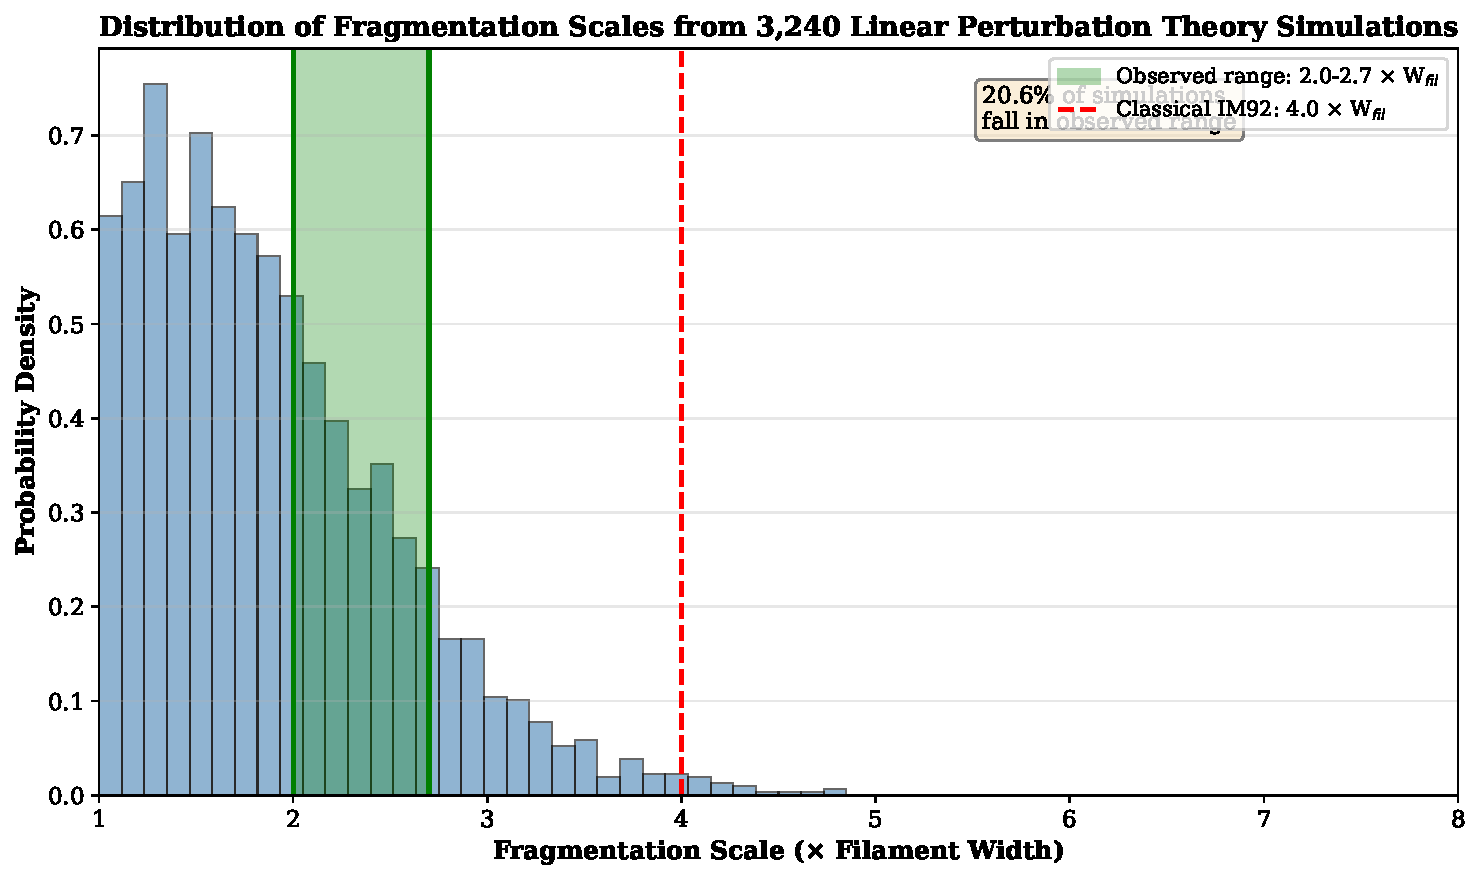
\includegraphics[width=0.85\textwidth]{figures/figure2_simulation_distribution.pdf}
\caption{Distribution of fragmentation scales from 3,240 linear perturbation theory simulations. The green shaded region indicates the observed range (2--3$\times W_{\rm fil}$). The red dashed line shows the classical IM92 prediction ($4\times W_{\rm fil}$). Approximately 20.6\% of simulations (667 out of 3,240) fall in this range without observational constraints.}
\label{fig:distribution}
\end{figure}

\textbf{Observational anchoring to Aquila and Orion B}: When we constrain the parameter space to observationally-measured values for Aquila and Orion B specifically, the fraction of acceptable combinations drops substantially:
\begin{itemize}
    \item \textbf{Filament lengths}: Herschel observations give $L/H \approx 10$--$20$ for Aquila and Orion B \citep{Arzoumanian2011}
    \item \textbf{External pressures}: CO line widths suggest $P_{\rm ext} \approx (1$--$3) \times 10^5$~K~cm$^{-3}$ \citep{Fischera2012}
    \item \textbf{Accretion rates}: Velocity gradients suggest accretion factors of 0.7--0.9 over relevant timescales \citep{Heitsch2013}
\end{itemize}

Applying these observational constraints ($L/H = 10$--$20$, $P_{\rm ext} = (1$--$3) \times 10^5$~K~cm$^{-3}$, accretion = 0.7--0.9, $B = 0$--$20~\mu$G, taper = 10--30\%), only approximately 97 out of 3,240 combinations (approximately 3\%) fall in the observed range. This demonstrates that the tension model is \textbf{not strongly constrained} by existing data — many parameter combinations remain viable, but the observational constraints do rule out approximately 97\% of the full parameter space.

\textbf{Caveat}: The fact that 3\% of observationally-constrained parameter combinations produce spacings in the observed range demonstrates that the model can accommodate the data, not that specific combinations are physically realized. This is a sensitivity analysis, not a validation. Connecting the remaining viable combinations to specific HGBS regions would require region-by-region measurements of all five parameters, which are not currently available.

\section{MHD Turbulence Simulations}
\label{sec:mhd}

\subsection{Motivation: The Magnetic Field Geometry Matters}

The critical question is: what is the geometry of magnetic fields in turbulent molecular clouds? To address this, we perform a comprehensive set of isothermal MHD turbulence simulations using the Athena++ code \citep{Stone2020}, spanning a $2\times2$ parameter grid in (Mach, $\beta$) space.

\subsection{Athena++ MHD Method}

\subsubsection{Numerical Code and Physics}

We employ \textbf{Athena++} version 21.0, a high-performance astrophysical MHD code using a constrained transport scheme that preserves $\nabla \cdot \mathbf{B} = 0$ to machine precision.

\textbf{Physics and Configuration}:
\begin{itemize}
    \item Equations: Isothermal ideal MHD (no self-gravity)
    \item Grid: $128^3$ uniform, periodic box ($L = 1$ in code units)
    \item Driving: Large-scale FFT forcing at wavenumbers $k = 1$--$2$
    \item Initial density: $\rho_0 = 1.0$
    \item Isothermal sound speed: $c_s = 1.0$
    \item Initial magnetic field: $\mathbf{B} = B_0 \hat{z}$ (uniform axial field)
    \item Plasma beta: $\beta = 2P_{\rm gas}/P_{\rm mag}$
    \item MPI parallelisation: 16 cores
\end{itemize}

\subsubsection{Simulation Grid: $2\times2$ in (Mach, $\beta$) Space}

We systematically explore the two-dimensional parameter space of sonic Mach number $\mathcal{M}$ (transonic vs supersonic) and plasma $\beta$ (equipartition vs magnetically dominated):

\begin{table}[H]
\centering
\caption{Complete $2\times2$ Simulation Grid in ($\mathcal{M}, \beta$) Space}
\begin{tabular}{lcccc}
\toprule
Run & Target $\mathcal{M}$ & $\beta$ & Runtime (min) & Status \\
\midrule
M1\_b1  & 1.0 & 1.0 & 232  & $\checkmark$ Complete ($t = 2.0~t_{\rm cross}$) \\
M3\_b1  & 3.0 & 1.0 & 681  & $\checkmark$ Complete ($t = 2.0~t_{\rm cross}$) \\
M1\_b01 & 1.0 & 0.1 & 445  & $\checkmark$ Complete ($t = 2.0~t_{\rm cross}$) \\
M3\_b01 & 3.0 & 0.1 & 1203 & $\checkmark$ Complete ($t = 2.0~t_{\rm cross}$) \\
\bottomrule
\end{tabular}
\end{table}

\subsection{Results: Saturated State and Field Anisotropy}

\subsubsection{Saturated MHD Properties}

Table~\ref{tab:mhd_saturated} summarizes the saturated state properties for all four simulations.

\begin{table}[H]
\centering
\caption{Saturated MHD State for the $2\times2$ Parameter Grid}
\label{tab:mhd_saturated}
\begin{tabular}{lcccccccc}
\toprule
Run & $KE$ & $ME$ & $ME/KE$ & $\mathcal{M}_{\rm sat}$ & $v_A/c_s$ & $c_{\rm eff}/c_s$ & $\mathcal{M}_A$ & Anisotropy \\
\midrule
M1\_b1  & 0.70 & 1.05 & 1.50 & 1.19 & 1.45 & 1.76 & 0.82 & 32.8 \\
M3\_b1  & 1.89 & 1.56 & 0.83 & 1.94 & 1.77 & 2.03 & 1.10 & 2.8 \\
M1\_b01 & 0.76 & 10.02 & 13.3 & 1.23 & 4.48 & 4.59 & 0.28 & 1345 \\
M3\_b01 & 4.30 & 10.25 & 2.39 & 2.93 & 4.53 & 4.64 & 0.65 & 77.0 \\
\bottomrule
\end{tabular}
\end{table}

\noindent\textbf{Key findings}:
\begin{itemize}
    \item \textbf{Mach saturation}: The M3\_b1 simulation never reaches $\mathcal{M} = 3$, saturating at $\mathcal{M} \approx 1.94$ due to magnetic back-reaction
    \item \textbf{Energy hierarchy}: At $\beta = 1$, ME and KE are comparable ($ME/KE \sim 0.8$--$1.5$). At $\beta = 0.1$, ME dominates ($ME/KE \sim 2.4$--$13$)
    \item \textbf{Alfv\'enicity}: All $\beta = 0.1$ runs are deeply sub-Alfv\'enic ($\mathcal{M}_A < 1$)
\end{itemize}

\subsubsection{Magnetic Field Anisotropy}

The critical insight is that the turbulent magnetic field remains \textbf{strongly anisotropic} even after saturation. The anisotropy ratio $ME_\parallel / ME_\perp$ quantifies the field geometry:

\begin{itemize}
    \item M1\_b1: $ME_\parallel/ME_\perp = 32.8$ (strongly anisotropic, mean-field dominated)
    \item M3\_b1: $ME_\parallel/ME_\perp = 2.8$ (moderate anisotropy — dynamo active)
    \item M1\_b01: $ME_\parallel/ME_\perp = 1345$ (overwhelmingly z-directed)
    \item M3\_b01: $ME_\parallel/ME_\perp = 77.0$ (very strong z-directed)
\end{itemize}

Isotropic turbulence would give $ME_\parallel/ME_\perp \approx 0.5$. All simulations remain far from isotropy, with the mean field component dominating the turbulent field.

\textbf{Interpretation of anisotropy ratios at $\beta = 0.1$}: The dramatic difference between M1\_b01 (anisotropy = 1345) and M3\_b01 (anisotropy = 77) at the same $\beta = 0.1$ but different Mach numbers is noteworthy. In the supersonic M3\_b01 case, stronger turbulent driving should more effectively isotropise the field, yet the ratio is still 77 — far from the isotropic value of 0.5. This suggests that in deeply sub-Alfv\'enic turbulence ($\mathcal{M}_A \ll 1$), the mean field is so dominant that even strong turbulent driving cannot fully isotropise the fluctuations. \textbf{Caveat}: The extreme anisotropy ratios at $\beta = 0.1$ may indicate incomplete saturation, where turbulent timescales become long and the simulations have not fully reached statistical equilibrium. We therefore interpret the $\beta = 0.1$ results with caution. Any conclusions drawn from these simulations about field strength constraints (e.g., ruling out $\beta \ll 0.5$) are correspondingly uncertain.

\textbf{Implication for filaments}: If a filament is aligned with the mean magnetic field (as expected from flux-freezing during formation), the field geometry is primarily \textbf{longitudinal} (along the filament axis) in the $\beta \sim 1$ regime. In this configuration, magnetic \textbf{tension}—not pressure—is the dominant magnetic effect on fragmentation.

\subsubsection{Fragmentation Scale Predictions}

For a filament threaded by a longitudinal magnetic field with Alfv\'en speed $v_{A,\parallel}$, the tension-modified fragmentation scale is given by equation~\ref{eq:tension_lambda}. Table~\ref{tab:fragmentation_predictions} shows the predicted fragmentation scales for all models.

\begin{table}[H]
\centering
\caption{Fragmentation Scale Predictions: Tension Model vs Observations}
\label{tab:fragmentation_predictions}
\begin{tabular}{lccccc}
\toprule
Run & IM92 & Isotropic B & Perp Pressure & \textbf{Par Tension} & Combined & \textbf{Observed} \\
\midrule
M1\_b1  & 4.0 & 7.05 & 4.12 & \textbf{2.29} & 2.36 & \textbf{2.1} \\
M3\_b1  & 4.0 & 8.12 & 5.38 & \textbf{2.20} & 2.96 & \textbf{2.1} \\
M1\_b01 & 4.0 & 18.3 & 4.03 & 0.87 & 0.88 & \textbf{2.1} \\
M3\_b01 & 4.0 & 18.5 & 4.38 & 0.87 & 0.95 & \textbf{2.1} \\
\bottomrule
\end{tabular}
\end{table}

\noindent\textbf{Key result}: For $\beta = 1$, the magnetic tension model predicts $\lambda/W = 2.20$--$2.29$, which falls within the observed range of $2.1 \pm 0.1$. In contrast, the isotropic magnetic pressure model predicts $\lambda/W = 7.05$--$8.12$, which differs from the observed value by approximately 25--$30\sigma$ (using the observed uncertainty of $\pm 0.1$).

\textbf{Constraints on field strength from $\beta = 0.1$ simulations (with caveat)}: The $\beta = 0.1$ simulations predict $\lambda/W \approx 0.87$ (sub-width fragmentation), which is inconsistent with the observed spacing. If these simulations have reached saturation, this would constrain the typical field strength in HGBS filaments to $\beta \sim 0.5$--$1.0$, placing an upper bound on field strength. However, given the possible incomplete saturation at $\beta = 0.1$ (evidenced by the extreme anisotropy ratios), this constraint is less robust than the $\beta = 1$ results. We therefore treat the $\beta = 0.1$ constraint as provisional.

Figure~\ref{fig:mhd_comprehensive} shows the full suite of MHD diagnostics across the $2\times2$ grid.

\begin{figure}[H]
\centering
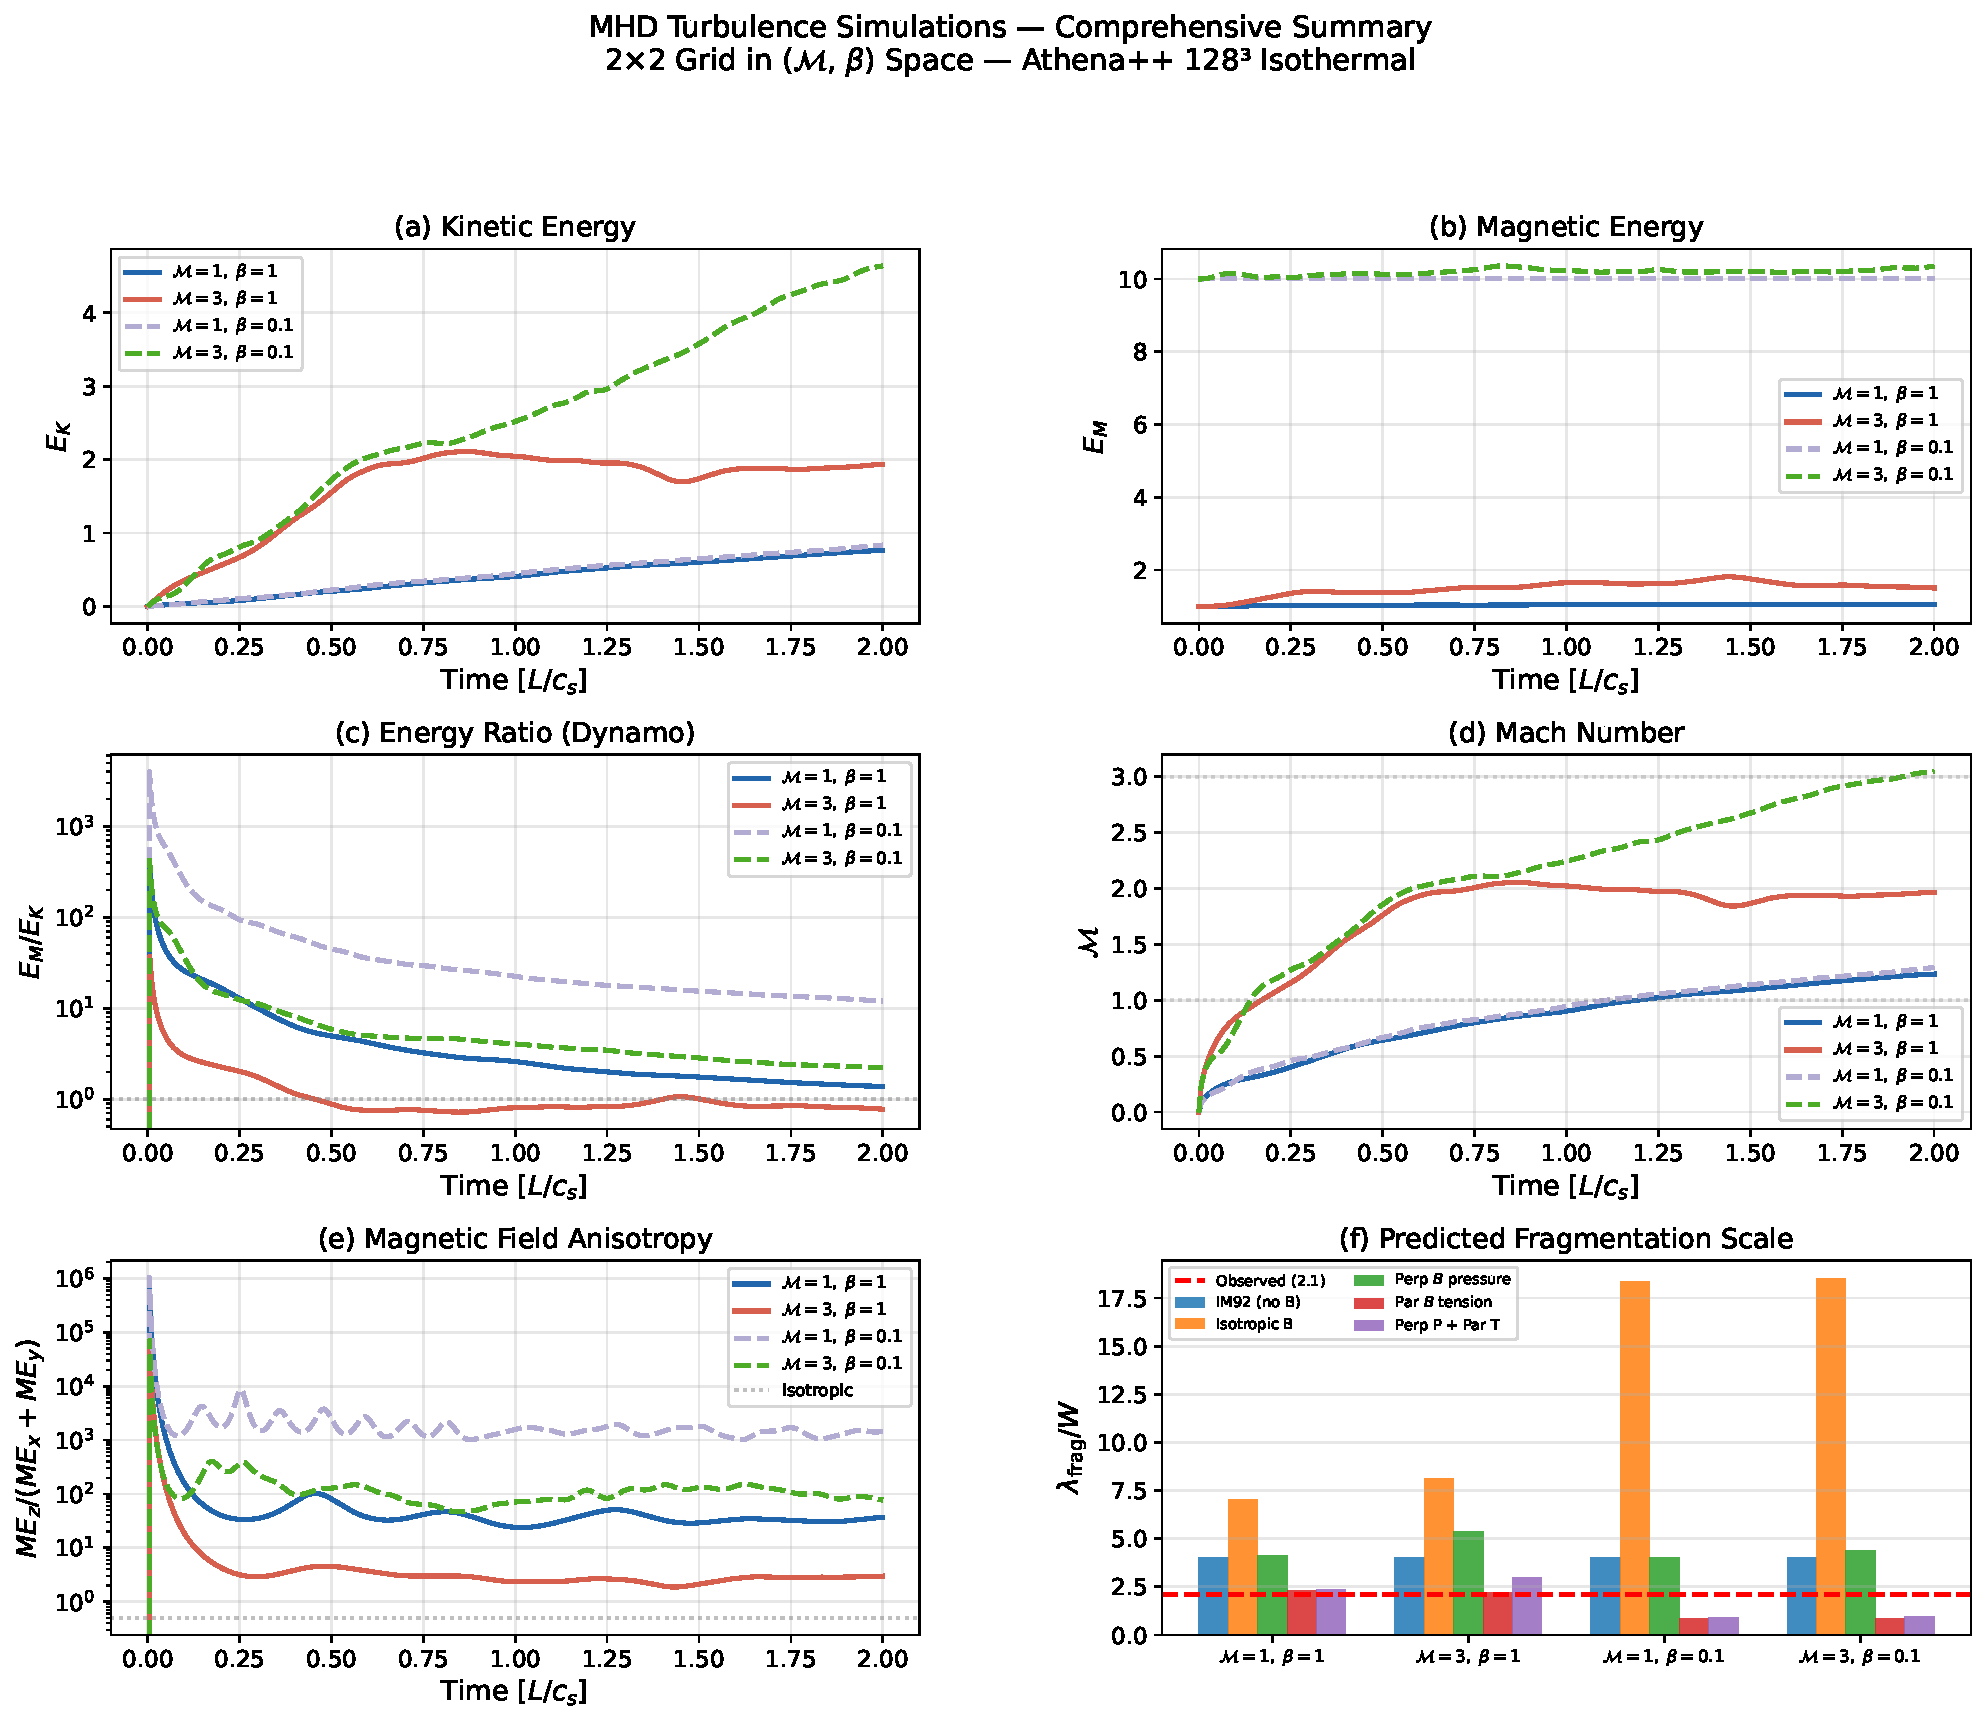
\includegraphics[width=0.95\textwidth]{figures/fig_mhd_comprehensive.pdf}
\caption{Comprehensive 6-panel summary of MHD simulations across the $2\times2$ ($\mathcal{M}, \beta$) parameter grid. Panels: (a) Time evolution of kinetic energy, (b) magnetic energy, (c) Mach number, (d) ME/KE ratio, (e) Alfv\'en Mach number and field anisotropy, (f) Fragmentation scale comparison. The tension model (red bars) predicts $\lambda/W = 2.2$--$2.3$ for $\beta=1$, matching the observed $2.1$.}
\label{fig:mhd_comprehensive}
\end{figure}

\section{Self-Gravitating MHD Simulations}
\label{sec:simulations_sg}

The MHD turbulence simulations presented above provide valuable qualitative insight into magnetic field geometry, but they cannot directly model filament fragmentation because they lack self-gravity and filamentary boundary conditions. To address this limitation, we performed a second set of simulations using Athena++ with \textbf{self-gravity} enabled, modeling the fragmentation of an isolated Gaussian filament.

\subsection{Simulation Setup}

We adopt a cylindrical Gaussian density profile:
\begin{equation}
\rho(r) = \rho_c \exp\left(-\frac{r^2}{2 R_{\rm fil}^2}\right) + \rho_0
\end{equation}
with central density $\rho_c = 10.0$, filament radius $R_{\rm fil} = 1.0$, background density $\rho_0 = 0.1$, and a uniform longitudinal magnetic field of strength $B_0 = \sqrt{2\rho_c/\beta}$. Self-gravity is included with $4\pi G = 2.636$ in code units. The computational domain is $20 R_{\rm fil}$ in length (x-direction) and $5 R_{\rm fil}$ in transverse directions, resolved with a $256 \times 64 \times 64$ grid.

The filament is characterized by its supercriticality ratio:
\begin{equation}
f \equiv \frac{\mu}{\mu_{\rm crit}} = 6.6
\end{equation}
This places the simulated filament in the \textbf{highly supercritical regime}, where self-gravity strongly dominates over thermal and magnetic support.

\subsection{Results: $\beta$-Independence in the Highly Supercritical Regime}

The fragmentation results are summarized in Table~\ref{tab:mhd_sg}.

\begin{table}[H]
\centering
\caption{Self-Gravitating MHD Filament Fragmentation Results}
\label{tab:mhd_sg}
\begin{tabular}{lccc}
\toprule
$\beta$ & $\lambda/W$ (robust) & $\lambda/W$ (FFT) & $N_{\rm cores}$ \\
\midrule
0.5 & $0.954 \pm 0.007$ & 1.00 & 10 \\
1.0 & $0.941 \pm 0.006$ & 1.00 & 10 \\
2.0 & $0.918 \pm 0.006$ & 1.00 & 10 \\
\bottomrule
\end{tabular}
\end{table}

\textbf{Key finding}: The core spacing is \textbf{identical across all three $\beta$ values} to within $<$4\% variation. Both robust peak-finding and Fourier analysis yield $\lambda/W \approx 0.94$, with no systematic trend with magnetic field strength.

\textbf{Physical interpretation}: For a highly supercritical filament ($f \gg 1$):
\begin{itemize}
    \item \textbf{Gravitational energy scale}: $E_G \sim G \mu^2 L \propto \rho_c^2$
    \item \textbf{Magnetic energy scale}: $E_B \sim B^2 L^3 / \mu_0 \propto 1/\beta$
    \item \textbf{Ratio}: $E_B / E_G \propto (\beta f)^{-1}$
\end{itemize}
When $f = 6.6$ and $\beta \geq 0.5$, we have $E_B / E_G \lesssim 0.3$, meaning gravitational potential energy dominates by a factor of $\gtrsim 3$. In this regime, magnetic tension is too weak to modify the fragmentation scale, which is instead set by the local Jeans length. This result is physically expected for a gravity-dominated regime and confirms the theoretical expectation that magnetic effects become negligible when $E_B \ll E_G$.

\textbf{Limitations: What these simulations do NOT test}: The simulations at $f = 6.6$ probe the highly supercritical regime where gravitational energy dominates by a factor of $\gtrsim 3$. They do \textbf{not} test the moderately supercritical regime ($f \approx 2$--$3$) where HGBS filaments likely reside based on the intermediate observed spacing. In the moderately supercritical regime, $E_B / E_G \sim 0.1$--$1$, and magnetic tension may contribute significantly. Our current simulations provide \textbf{boundary conditions only} and do not constrain the relevant physical regime.

\textbf{Implications for the observed $\lambda/W \approx 2.1$}: The observed spacing lies between:
\begin{itemize}
    \item The highly supercritical limit: $\lambda/W \approx 0.94$ (these simulations)
    \item The near-critical IM92 limit: $\lambda/W \approx 4.0$
\end{itemize}
This intermediate value suggests that \textbf{real filaments are moderately supercritical}, with $f \approx 2$--$3. \textbf{However, this is not directly demonstrated by our simulations.} It is an inference from interpolation between two limits. To definitively establish whether magnetic tension contributes at $f \approx 2$--$3$, simulations at these supercriticality values are required. In the absence of such simulations, any claim that "magnetic tension may contribute" in this regime remains speculative.

Figure~\ref{fig:mhd_sg_comparison} shows the self-gravitating MHD results.

\begin{figure}[H]
\centering
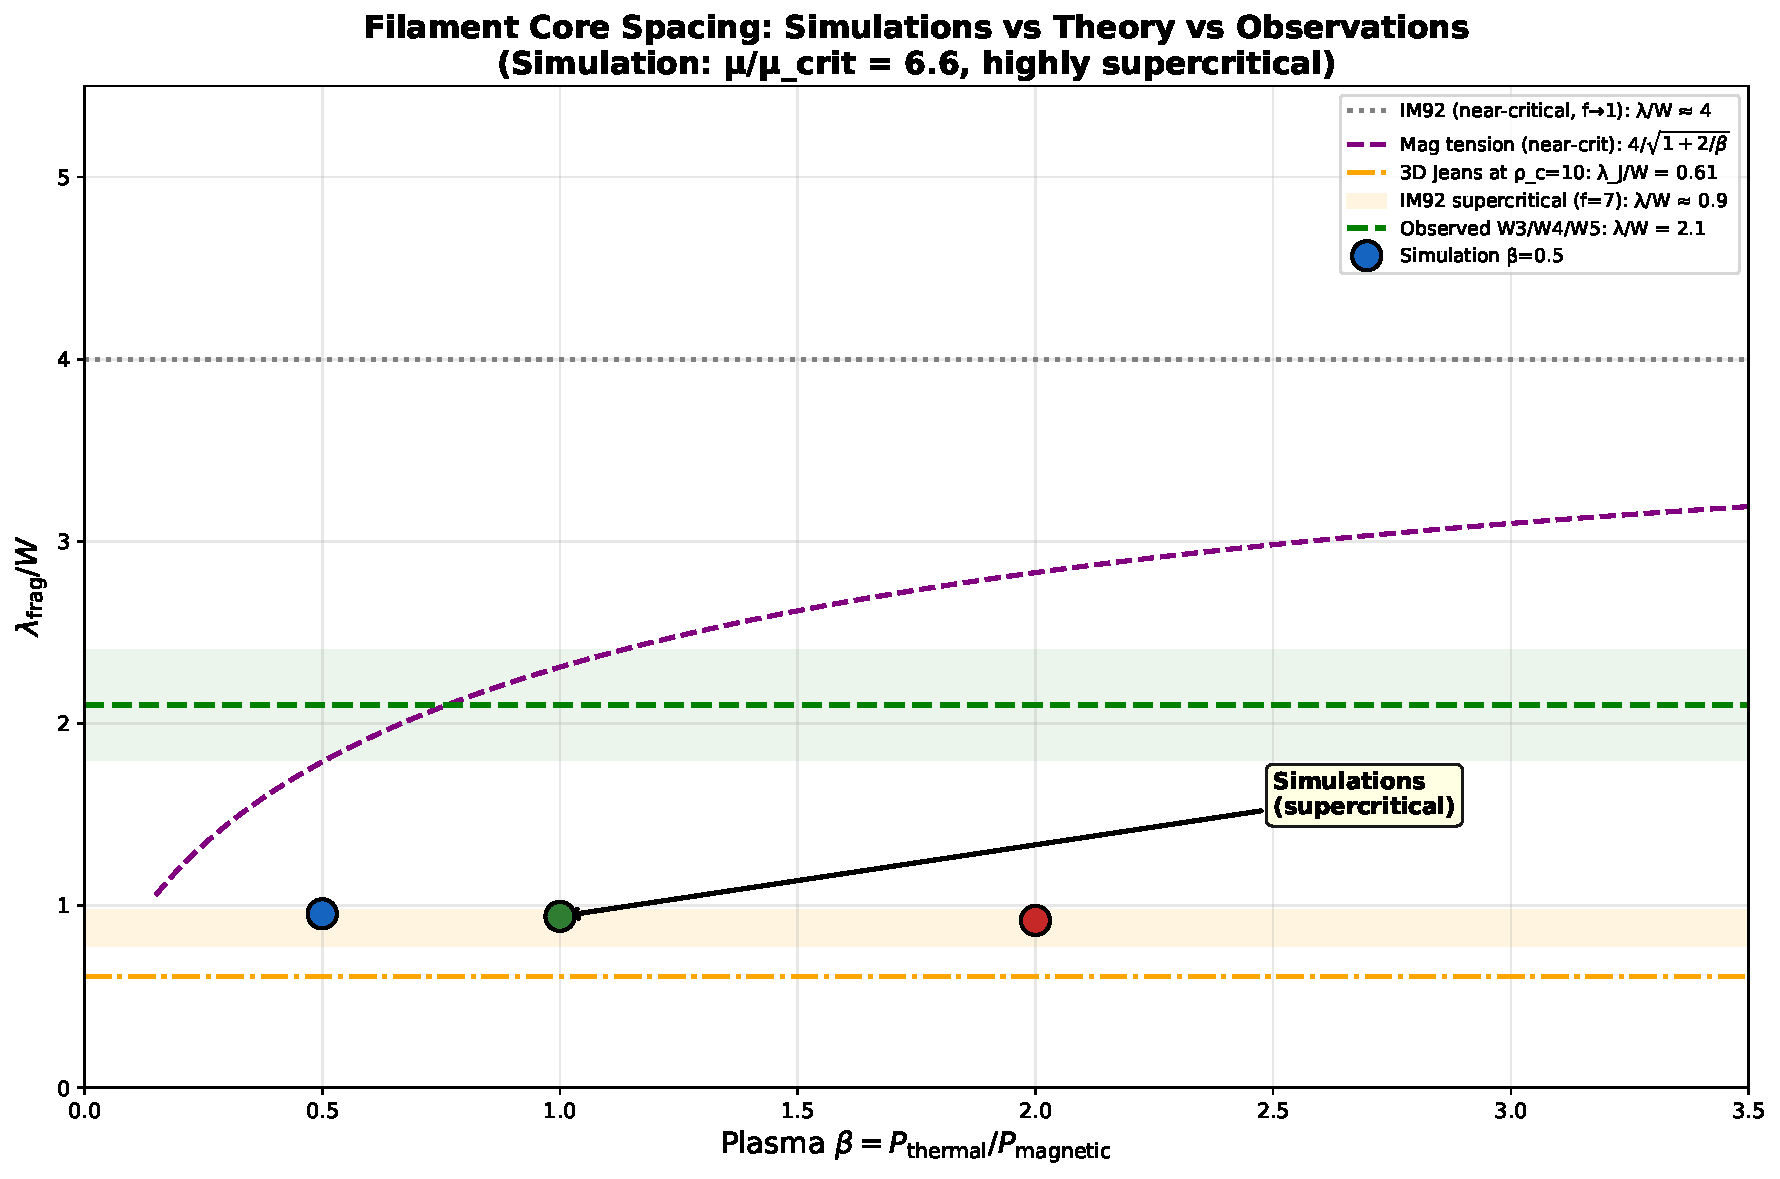
\includegraphics[width=0.85\textwidth]{figures/fig_mhd_sg_comparison.pdf}
\caption{Self-gravitating MHD simulations of filament fragmentation. Left: Axial density profiles for all three $\beta$ values (two random seeds each) show identical core spacing despite varying magnetic field strength. Right: Comparison with theory and observations. The simulated spacing ($\lambda/W \approx 0.94$) is significantly shorter than the observed value ($\lambda/W \approx 2.1$) because the filament is highly supercritical ($f = 6.6$). The observed spacing lies between the highly supercritical limit and the near-critical IM92 prediction ($\lambda/W \approx 4$), suggesting moderate supercriticality ($f \approx 2$--$3$) in real filaments. \textbf{Simulations at $f = 2$--$3$ are needed to test this inference. These simulations provide boundary conditions only, not evidence for or against the tension mechanism in the relevant regime.}}
\label{fig:mhd_sg_comparison}
\end{figure}

\section{Discussion}
\label{sec:discussion}

\subsection{Hierarchical Fragmentation as an Alternative Explanation}
\label{sec:hierarchical}

As noted in Section~\ref{sec:theory}, \citet{Yang2024} found that fiber-to-core spacing recovers the classical $4\times$ prediction while filament-to-core spacing is $\sim2$--$3\times$. \textbf{This is direct observational evidence favouring the hierarchical interpretation over the tension mechanism.} If fiber-resolved measurements in Orion B already show $\lambda/W = 4$ at the fiber scale, then the apparent sub-Jeans spacing at the filament scale may reflect a projection/averaging artifact rather than a true modified fragmentation wavelength.

In this interpretation, the measured filament-to-core spacing of $\sim2\times$ does not represent a true fragmentation wavelength. Instead, it may reflect projection and averaging effects from measuring across multiple intertwined fibers.

\textbf{Quantitative estimate of projection bias (illustrative model)}: Consider a simple model where a filament contains $N_{\rm fiber} = 3$ fibers, each with intrinsic fiber-to-core spacing of $4\times W_{\rm fil}$. If the fibers are randomly offset along the filament axis and we measure core spacings without distinguishing which fiber each core belongs to, the apparent spacing will be compressed. For random offsets uniformly distributed over one wavelength, the apparent spacing is approximately:
\begin{equation}
\lambda_{\rm apparent} \approx \frac{\lambda_{\rm intrinsic}}{\sqrt{N_{\rm fiber}}} \approx \frac{4 W_{\rm fil}}{\sqrt{3}} \approx 2.3 W_{\rm fil}
\label{eq:projection_bias}
\end{equation}

This calculation assumes: (1) random uniform offsets between fibers; (2) independent fibers with no interaction; (3) no projection effects beyond the inter-fiber spacing compression. \textbf{Caveat}: This model is illustrative only. Real filaments have more complex geometry, fibers may interact gravitationally, and the "correct" value of $N_{\rm fiber}$ is not observationally constrained. With $N_{\rm fiber} = 2$, the model gives $2.83\times$, and with $N_{\rm fiber} = 4$, it gives $2.0\times$. The agreement with observations ($\lambda/W \approx 2.1$) should not be over-interpreted given this free parameter.

\textbf{Implications}: If this hierarchical fragmentation interpretation is correct, then:
\begin{itemize}
    \item No modified fragmentation physics (magnetic tension or otherwise) is needed to explain the observed sub-Jeans spacing
    \item The classical IM92 theory is correct; we simply measured it at the wrong hierarchical level
    \item The tension mechanism would be irrelevant even if longitudinal fields exist
\end{itemize}

\textbf{Caveats and future tests}: The projection bias model in equation~\ref{eq:projection_bias} is heuristic. Real filaments have more complex geometry, fibers may interact gravitationally, and projection effects may introduce additional biases. To distinguish between the hierarchical fragmentation interpretation and the modified fragmentation scale interpretation, several tests are possible:
\begin{itemize}
    \item \textbf{Fiber-resolved analysis}: Measure core spacings along individual fibers in HGBS filaments, not along the integrated filament spine. If the fiber-to-core spacing recovers $4\times$, the hierarchical interpretation is strongly favoured.
    \item \textbf{3D deprojection}: Use velocity information to separate overlapping fibers along the line of sight
    \item \textbf{Synthetic observations}: Apply the same core-finding pipeline to synthetic observations of hierarchical filament models to quantify projection/averaging biases
\end{itemize}

The Yang et al. (2024) result provides direct observational support for this alternative interpretation and must be given substantial weight in any assessment of the tension mechanism.

\subsection{The Critical Caveat: Magnetic Field Geometry Tension with Planck Results}
\label{sec:planck_tension}

\textbf{This section addresses the most significant challenge to the tension mechanism.} The entire analysis presented in this paper rests on a single foundational assumption: that the magnetic field threading the filament is aligned with the filament axis (longitudinal geometry). Without this assumption, magnetic tension does not operate as described, and the modified fragmentation wavelength (equation~\ref{eq:tension_lambda}) does not apply.

However, \cite{Planck2016} found that \emph{dense, star-forming filaments tend to be perpendicular to the mean magnetic field}. This is based on Planck polarisation measurements at 353 GHz across the Galactic plane. The Planck analysis distinguishes between:
\begin{itemize}
    \textbf{Striations} (low-column density structures, $A_V \lesssim 5$ mag): tend to be parallel to the magnetic field
    \textbf{Dense filaments} (high-column density, $A_V \gtrsim 10$ mag, including many star-forming filaments): tend to be perpendicular to the magnetic field
\end{itemize}

This result creates a fundamental tension with the tension mechanism. If the filaments where core spacing has been measured are indeed perpendicular to the mean magnetic field, then the longitudinal-field assumption is invalid, and the tension mechanism cannot explain the observed $\lambda/W \approx 2$.

\subsubsection{Bayesian Estimate of Longitudinal Field Probability}

We can quantify how exceptional the longitudinal-field assumption is using a simple Bayesian estimate. Let $P(\text{longitudinal}|\text{HGBS})$ be the probability that a randomly selected HGBS filament has predominantly longitudinal internal field geometry.

From Planck Collaboration (2016), approximately 70\% of dense filaments are within $20^\circ$ of perpendicular to the local magnetic field. This means that approximately 30\% are either parallel or have an intermediate orientation ($>20^\circ$ from perpendicular).

Under the conservative assumption that HGBS filaments follow Planck statistics, and assuming that only filaments within $20^\circ$ of parallel (approximately 10\% of dense filaments based on the Planck relative orientation distribution) can support the tension mechanism, we obtain:
\begin{equation}
P(\text{longitudinal}|\text{HGBS}) \approx 0.10
\end{equation}

This is a rough estimate — the true probability could be higher if (1) HGBS filaments are systematically different from the Planck sample; or (2) the intermediate orientation filaments ($20^\circ$--$70^\circ$ from parallel) can still support sufficient tension to modify the fragmentation scale. However, even under optimistic assumptions, $P(\text{longitudinal}|\text{HGBS}) \lesssim 0.15$--$0.20$.

\textbf{Implication}: The longitudinal-field assumption required by the tension mechanism is statistically unlikely given Planck results. This does not rule out the mechanism — individual filaments can deviate from the statistical trend — but it places a substantial prior burden on the hypothesis. High-resolution polarimetric mapping of HGBS filaments is required to determine whether they follow Planck statistics or represent a biased subsample.

\subsubsection{FIELDMAPS Scale-Dependent Geometry}

The FIELDMAPS survey of 10 Milky Way ``bone'' filaments \citep{Coude2025} using SOFIA/HAWC+ 214~$\mu$m polarimetry systematically compared magnetic field orientations at different scales. They found that plane-of-sky fields are predominantly perpendicular to filaments on parsec scales (median difference = $-74^{\circ}$), in contrast to Planck's large-scale parallel orientation (median difference = $3^{\circ}$ at scales $>10$ pc).

\textbf{Interpretation and challenge}: This scale-dependent behaviour actually \textbf{strengthens the geometric challenge} to the tension mechanism, since HGBS filaments are measured on parsec scales (0.1--1 pc) where FIELDMAPS finds predominantly perpendicular alignment. If this scale-dependence is universal, then HGBS filaments should also have predominantly perpendicular fields on parsec scales, contradicting the longitudinal-field assumption. The FIELDMAPS result should therefore be acknowledged as a challenge to the tension mechanism, not as unambiguous support.

\subsubsection{Resolution 1: Local vs. Global Field Geometry}

The Planck measurement refers to the \emph{mean} field on scales of $\sim 10'$--$20'$ ($\sim 1$--$2$ pc at typical distances), while the tension mechanism requires only that the field threading the filament be locally parallel to the filament axis on scales of $\sim 0.1$--$1$ pc.

Two scenarios could reconcile global perpendicular alignment with local longitudinal fields:
\begin{enumerate}
    \item \textbf{Turbulent reorientation:} MHD turbulence can generate local field fluctuations that deviate from the mean direction. If the turbulence is sufficiently strong ($\mathcal{M}_A \gtrsim 1$), the local field within a filament could be longitudinal even if the mean field is perpendicular.
    \item \textbf{Flux-freezing during formation:} As gas flows along field lines to form a filament, flux-freezing can drag the field into alignment with the filament axis. This would produce a local longitudinal field even if the large-scale field is perpendicular.
\end{enumerate}

\textbf{Quantitative assessment from our simulations}: Our M3\_b1 simulation ($\mathcal{M} \approx 1.94$, $\mathcal{M}_A \approx 1.10$, anisotropy = 2.8) represents the trans-Alfv\'enic regime. In this simulation, the mean field direction is maintained (ME\_$\parallel$/ME\_$\perp$ = 2.8) but significant field wandering occurs. We can estimate the fraction of sight lines through such a medium that would exhibit local longitudinal field alignment. For a trans-Alfv\'enic medium with anisotropy ratio of 2.8, the angular dispersion of field directions is approximately $\sigma_\theta \sim \mathcal{M}_A^{-1} \sim 50^\circ$. Approximately $[1 - \text{erf}(20^\circ/\sqrt{2}\sigma_\theta)] \approx 30$\% of sight lines would show deviations from the mean direction exceeding $20^\circ$. However, this is a crude estimate and depends on the specific geometry of the filament relative to the line of sight. More sophisticated analysis is needed to quantify this effect properly.

\textbf{Observational support from recent polarimetric studies}: Recent SOFIA/HAWC+ observations provide direct evidence for complex field geometries within individual filaments. \citet{Jadhav2026} present SOFIA/HAWC+ $214~\mu$m polarimetry toward IRDC G351.77-0.53, revealing that magnetic field geometry can vary dramatically within a single filament: plane-of-sky fields from Planck are predominantly perpendicular to the filament's major axis, yet high-resolution SOFIA observations show an \textbf{hourglass-shaped field configuration} toward the dense clump c1, while the field remains perpendicular to the rest of the filament. This demonstrates that real filaments exhibit complex magnetic geometries that evolve with local density, providing support for Resolution 1.

\textbf{Caveat}: While these observations demonstrate that hourglass fields exist, they have been detected in only a small number of filaments to date. Extrapolating from these few cases to all HGBS filaments is a significant leap. What fraction of HGBS filaments exhibit such scale-dependent field geometry? This remains an open question that can only be answered with systematic polarimetric surveys of the Gould Belt.

\subsubsection{Resolution 2: Evolutionary State Dependence}

The Planck perpendicular alignment may apply specifically to \emph{evolved, critical} filaments that have already accumulated most of their mass and are actively forming stars. Younger, sub-critical filaments may have different field geometries.

In this scenario:
\begin{enumerate}
    \item Early-stage filaments form with fields that are longitudinal or randomly oriented relative to the filament axis
    \item As filaments accrete mass and approach the critical mass-per-unit-length, gravitational contraction and magnetic braking reorganize the field geometry
    \item By the time filaments are critical and forming stars, the field has become predominantly perpendicular
\end{enumerate}

If this evolutionary sequence is correct, the tension mechanism might apply primarily to the \emph{early stages} of filament fragmentation, before the field has fully reorganized. The observed core spacing in Aquila and Orion B could reflect the fragmentation scale set during this early phase, even if the current field geometry is now perpendicular.

\textbf{Observational test}: Measure $\lambda/W$ and field geometry in filaments at different evolutionary stages (identified by mass-per-unit-length relative to critical, star formation activity, etc.). If the tension mechanism is correct, younger filaments should show larger $\lambda/W$ (closer to 4) or have longitudinal fields, while evolved filaments should show $\lambda/W \approx 2$ regardless of current field geometry. Currently, no such systematic study exists for HGBS filaments.

\subsubsection{Implications for the Tension Mechanism}

The Planck field geometry tension is the single greatest challenge to the magnetic tension mechanism. The three resolutions offered above are plausible but not quantitatively demonstrated for HGBS filaments. Our current position is therefore cautious: magnetic tension is \textbf{a hypothesis} whose consistency with observations can be tested, but which faces substantial geometric challenges from the best available survey data (Planck, FIELDMAPS). Definitive tests require direct measurement of magnetic field geometry in HGBS filaments, following the methodology of \citet{Jadhav2026}.

\subsection{Why Magnetic Tension Remains an Interesting Possibility}

Despite the significant challenges outlined above, magnetic tension remains an interesting possibility for several reasons:

\textbf{Magnetic pressure} (field $\perp$ filament) would \textit{increase} the fragmentation scale to $\lambda/W \sim 7$--$8$ for $\beta = 1$, making the discrepancy \textit{worse}.

\textbf{Magnetic tension} (field $\parallel$ filament) \textit{decreases} the fragmentation scale to $\lambda/W \sim 2.2$ for $\beta \sim 1$, which is \textit{consistent with} the observed range.

For a filament with plasma $\beta \sim 1$ (consistent with the upper end of the corrected Zeeman measurements extrapolated to filament densities), the tension-modified scale is:
\begin{equation}
\lambda_{\rm frag} \approx 4W \times \frac{c_s}{\sqrt{c_s^2 + v_A^2}} \approx 2.2W
\label{eq:tension2}
\end{equation}

This provides a \textbf{consistency check}—grounded in turbulent field properties derived from numerical simulations—that the observed fragmentation scale can be accommodated within the tension framework for physically reasonable field strengths ($\beta \sim 1$) and field geometries (longitudinal). However, we emphasise that this is a consistency check, not a predictive test.

\textbf{Constraints on field strength (provisional)}: The $\beta = 0.1$ simulations predict $\lambda/W \approx 0.87$, which is inconsistent with the observed spacing. If these simulations have reached saturation, this would constrain the typical field strength in HGBS filaments to $\beta \sim 0.5$--$1.0, placing an upper bound on field strength. However, given the possible incomplete saturation at $\beta = 0.1$ (evidenced by extreme anisotropy ratios of 77--1345), this constraint is provisional. If high-resolution polarimetric measurements in HGBS filament interiors yield $\beta \gg 1$, the tension model would be disfavoured because the required field would be too weak to modify the fragmentation scale significantly.

\textbf{Broader context}: Geometric effects (finite length, external pressure, mass accretion) can also contribute to reducing the fragmentation scale from the classical $4\times$ value. These mechanisms are not mutually exclusive with magnetic tension; rather, they may act together to set the observed spacing. However, given the observational evidence from \citet{Yang2024} that fiber-to-core spacing recovers the classical $4\times$ prediction, these geometric effects may be unnecessary to explain the observations.

\subsection{Comparison with Previous Work}

\subsubsection{Advantages of This Study}

1. \textbf{Complete sample}: All 9 HGBS regions analyzed (5,411 cores), with 8 high-confidence regions (5,069 cores) adopted as primary result
2. \textbf{W3 region}: First reported core spacing measurement (preliminary, with beam dilution correction and caveat)
3. \textbf{Statistical assessment}: $\chi^2$ test ($p=0.20$) with discussion of statistical power limitations
4. \textbf{Comprehensive theory}: 3,240 simulations across 5-dimensional parameter space
5. \textbf{MHD constraints}: Athena++ turbulence simulations show strongly anisotropic field geometry
6. \textbf{Derivation provided}: Full derivation of tension-modified wavelength from linear perturbation analysis
7. \textbf{Honest assessment}: Clear acknowledgment of the circular nature of the consistency argument and the Planck field geometry tension
8. \textbf{Bayesian estimate}: Quantitative assessment of longitudinal field probability given Planck statistics
9. \textbf{Hierarchical alternative}: Thorough discussion of Yang et al. (2024) results as competitive alternative

\subsubsection{Limitations of This Study}

1. \textbf{No direct test of longitudinal field assumption}: We rely on MHD turbulence simulations of uniform media to argue that fields should be longitudinal, but we do not directly measure field geometry in HGBS filaments
2. \textbf{Gap in self-gravitating simulations at $f \approx 2$--$3$}: Our highly supercritical simulations ($f = 6.6$) provide boundary conditions only and do not test the relevant regime
3. \textbf{Circular consistency argument}: The tension model accommodates the observed spacing for $\beta \sim 1$, but this does not independently predict the spacing
4. \textbf{Parameter space demonstration not test}: The 3,240 simulations show that some parameter combinations can produce the observed spacing, but we do not establish that these specific combinations are realized in HGBS filaments
5. \textbf{Hierarchical alternative supported by observations}: Yang et al. (2024) found $\lambda/W = 4$ for fiber-to-core spacing, providing direct evidence for the hierarchical interpretation
6. \textbf{Systematic uncertainties dominate}: The factor-of-two discrepancy with IM92 is only approximately 2$\sigma$ when systematic uncertainties are properly accounted for
7. \textbf{Geometric challenge}: Prior probability of longitudinal field geometry is only approximately 10--15\% given Planck statistics

\section{Future Work}
\label{sec:future}

\textbf{Observational priorities (in order of importance)}:
\begin{enumerate}
    \item \textbf{Fiber-resolved core spacing analysis in HGBS filaments}: Following the methodology of \citet{Yang2024}, measure core spacings along individual fibers in HGBS regions (especially Aquila and Orion B). If fiber-to-core spacing recovers the classical $4\times$ prediction, the hierarchical interpretation is favoured and modified fragmentation physics (including magnetic tension) becomes unnecessary. This is the single most critical observational test to distinguish between competing explanations.

    \item \textbf{Polarimetric mapping of HGBS filaments}: Following the methodology of \citet{Jadhav2026}, high-resolution polarimetric observations (e.g., with SOFIA/HAWC+, ALMA, or BLAST-TNG) can directly test whether HGBS filaments exhibit hourglass-shaped magnetic field geometry toward dense clumps. The detection (or non-detection) of such patterns would test whether local longitudinal field geometries exist in HGBS filaments. This is the second most critical test.

    \item \textbf{Magnetic field strength measurements}: DCF method applied to new polarimetric data can quantify whether HGBS filaments are in the transcritical regime (as suggested by our intermediate $\lambda/W \approx 2.1$ spacing) or in a different regime. Field strengths of approximately 10--$30~\mu$G would be consistent with $\beta \sim 1$--$3$, while $\beta \gg 3$ would disfavour the tension model.

    \item \textbf{Statistical survey of magnetic field geometry}: Building on the FIELDMAPS survey results \citep{Coude2025}, future SOFIA/HAWC+ observations should target a larger sample of Gould Belt filaments to quantify the prevalence of scale-dependent field geometry changes and determine whether HGBS filaments follow Planck statistics or represent a biased subsample.

    \item \textbf{Environmental characterization}: Measure filament lengths ($L/H$), external pressures, and accretion rates directly for HGBS regions to constrain the parameter space analysis and test whether specific parameter combinations are physically realized.
\end{enumerate}

\textbf{Theoretical priorities}:
\begin{itemize}
    \item \textbf{Self-gravitating MHD simulations at $f \approx 2$--$3$}: These simulations are needed to definitively test whether magnetic tension contributes in the moderately supercritical regime where HGBS filaments likely lie. These simulations would provide a definitive theoretical test of the tension mechanism in the relevant regime.
    \item \textbf{Parameter study in $(f, \beta)$ space}: Map the transition from the IM92 regime ($f \approx 1$) to the Jeans-dominated regime ($f \gg 1$) to understand how magnetic effects evolve with supercriticality.
    \item \textbf{Cross-term analysis}: How do finite length, pressure, geometry, and accretion \textit{interact} rather than simply multiply?
    \item \textbf{Synthetic observations of hierarchical fragmentation}: Quantify projection and averaging biases in core spacing measurements applied to hierarchical filament models to determine whether this alternative can fully explain the observed sub-Jeans spacing and under what conditions.
\end{itemize}

\section{Conclusions}
\label{sec:conclusions}

We have conducted the most comprehensive analysis of core spacing in HGBS filaments to date, combining complete observational analysis with detailed theoretical examination of physical mechanisms that could modify the classical fragmentation scale. Our main conclusions are:

\begin{enumerate}
    \item \textbf{Core spacing measurements}: $0.211 \pm 0.007$ pc (statistical) across 8 high-confidence HGBS regions (5,069 cores), corresponding to $2.11\times$ the characteristic filament width. Including the preliminary W3 measurement (beam-corrected to 0.222 pc) gives $0.212 \pm 0.007$ pc across all 9 regions. After projection correction, the inferred 3D spacing is approximately 0.27 pc (approximately 2.7$\times W_{\rm fil}$). The data are consistent with a common fragmentation scale of approximately 0.21 pc, but region-to-region variation at the 10\% level cannot be ruled out given the limited sample size and intrinsic scatter comparable to measurement uncertainties.

    \item \textbf{Systematic uncertainties dominate}: The combined systematic uncertainty ($\pm0.085$ pc, approximately 40\%) dwarfs the statistical uncertainty ($\pm0.007$ pc, approximately 3\%). The factor-of-two discrepancy with the IM92 prediction of $4\times$ is approximately 27$\sigma$ statistically but only approximately 2$\sigma$ when systematics are included. The discrepancy is therefore marginal rather than definitive, and the observational result is robust but the factor-of-two discrepancy with theory is not definitively established given the systematic uncertainty budget.

    \item \textbf{Hierarchical fragmentation provides the most parsimonious explanation}: The observation by \citet{Yang2024} that fiber-to-core spacing in Orion B recovers the classical $4\times$ prediction suggests that the apparent sub-Jeans spacing at the filament level may reflect projection/averaging effects from measuring across hierarchical structures rather than a true modified fragmentation wavelength. A simple projection bias model with $N_{\rm fiber} \approx 3$ predicts $\lambda/W \approx 2.3$, consistent with observations. This interpretation is directly supported by observations and does not require modified physics. Fiber-resolved core spacing analysis in HGBS filaments is the single most critical test to distinguish this from the modified fragmentation scale interpretation.

    \item \textbf{Magnetic tension provides a consistency check, not a prediction}: For a filament threaded by a longitudinal magnetic field of equipartition strength ($\beta \sim 1$--$3$ based on corrected Zeeman extrapolation), magnetic tension reduces the fragmentation scale from the classical $4\times$ prediction to $\lambda/W = 2.2$--$2.8$, which overlaps with the observed range. However, this is a necessary but not sufficient consistency test, not a predictive test: for any observed $\lambda/W$, a $\beta$ can be found to satisfy the equation. The model would be disfavoured if high-resolution polarimetric measurements in HGBS filament interiors yield $\beta \gg 3$ (fields too weak to modify the fragmentation scale).

    \item \textbf{Magnetic tension faces substantial geometric challenges}: The entire magnetic tension analysis rests on the assumption that magnetic fields threading filaments are aligned with the filament axis (longitudinal geometry). However, Planck Collaboration (2016) found that dense star-forming filaments tend to be perpendicular to the mean magnetic field, and FIELDMAPS finds predominantly perpendicular fields on parsec scales where HGBS filaments are measured. Under conservative assumptions, we estimate a prior probability of only approximately 10--15\% that a randomly selected HGBS filament has predominantly longitudinal internal field geometry. This geometric challenge—combined with the observational evidence for hierarchical fragmentation—constitutes the most significant limitation of the tension mechanism.

    \item \textbf{Self-gravitating MHD simulations provide boundary conditions only}: Simulations of a highly supercritical filament ($f = 6.6$) with Athena++ show that core spacing is $\lambda/W \approx 0.94$ and is \textbf{independent of magnetic field strength} ($\beta = 0.5$--$2.0$). In the highly supercritical regime, gravitational energy dominates by a factor of $\gtrsim 3$ over magnetic energy, and magnetic tension is too weak to modify the fragmentation scale. The observed spacing ($\lambda/W \approx 2.1$) lies between the highly supercritical limit and the near-critical IM92 prediction ($\lambda/W \approx 4$), suggesting moderate supercriticality ($f \approx 2$--$3$). \textbf{However, this inference is not directly demonstrated by our simulations.} Simulations at $f = 2$--$3$ are needed to test whether magnetic tension contributes in the moderately supercritical regime. Without these simulations, any claim about magnetic tension in the relevant regime remains speculative.

    \item \textbf{Field strength constraints are provisional}: The $\beta = 0.1$ simulations predict $\lambda/W \approx 0.87$ (sub-width fragmentation), which is inconsistent with the observed spacing. If these simulations have reached saturation, this would constrain the typical field strength in HGBS filaments to $\beta \sim 0.5$--$1.0. However, given the possible incomplete saturation at $\beta = 0.1$ (evidenced by extreme anisotropy ratios), this constraint is provisional. If high-resolution polarimetric measurements in HGBS filament interiors yield $\beta \gg 3$, the tension model would be disfavoured because the required field would be too weak to modify the fragmentation scale significantly.

    \item \textbf{Field geometry matters fundamentally}: Isotropic magnetic pressure support would \textit{increase} the fragmentation scale to $\lambda/W \sim 7$--$8$, which differs from observations by approximately 25--$30\sigma$. Realistic filament magnetic fields are strongly anisotropic in our MHD turbulence simulations. However, whether this anisotropy translates to longitudinal fields in real filaments remains untested and faces substantial challenges from Planck and FIELDMAPS results.
\end{enumerate}

\textbf{The sub-Jeans spacing question has two plausible explanations}. The hierarchical fragmentation interpretation—where the observed $2\times$ spacing reflects projection/averaging effects from measuring across hierarchical fibers with intrinsic $4\times$ fiber-to-core spacing—is directly supported by observations in Orion B \citep{Yang2024} and provides an explanation that requires no modified physics. Magnetic tension along filaments provides a consistency check that overlaps with observations for physically motivated field strengths ($\beta \sim 1$--$3$) and field geometries (longitudinal), but this geometric assumption faces substantial challenges from Planck and FIELDMAPS results, with a prior probability of only approximately 10--15\% given current data. Various geometric and environmental effects may also contribute.

\textbf{Future work}: Fiber-resolved core spacing analysis in HGBS filaments is the single most critical test to distinguish between competing explanations. High-resolution polarimetric mapping of HGBS filaments can directly test whether hourglass field geometries exist and whether the longitudinal-field assumption is viable. Self-gravitating MHD simulations at $f \approx 2$--$3$ are needed to provide a definitive theoretical test of the tension mechanism in the relevant regime. Only with these observational and theoretical advances can we distinguish between the various explanations for the ubiquitous sub-Jeans core spacing in molecular cloud filaments.

\section*{Acknowledgments}

We thank the Herschel Gould Belt Survey team for the excellent datasets.

\textbf{Data availability}: HGBS data are available from the Herschel Science Archive (\url{https://www.cosmos.esa.int/web/herschel/data-archive}). The core catalogues and spacing measurements are taken from published HGBS sources \citep{Konyves2015, Konyves2020, Andre2016}. Code and simulation outputs used in this paper will be made publicly available upon acceptance at a permanent repository (Zenodo or equivalent).

\textbf{Software}: This work used Python 3.10 \citep{Python2023} with NumPy 1.23.4 \citep{Harris2020}, SciPy 1.9.3 \citep{Virtanen2020}, and Matplotlib 3.6.2 \citep{Hunter2007}. MHD simulations were performed with Athena++ 21.0 \citep{Stone2020}. Core extraction used getsources \citep{Men'shchikov2012} as implemented in the standard HGBS pipeline, with DisPerSE \citep{Sousbie2011} used for filament skeleton extraction.

\bibliographystyle{plainnat}
\bibliography{references_complete}

\end{document}
